\documentclass[a4paper, USenglish, cleveref]{lipics-v2021}
% Necessary for tikz to work on arxiv
\pdfoutput=1
%This is a template for producing LIPIcs articles. 
%See lipics-v2021-authors-guidelines.pdf for further information.
%for A4 paper format use option "a4paper", for US-letter use option "letterpaper"
%for british hyphenation rules use option "UKenglish", for american hyphenation rules use option "USenglish"
%for section-numbered lemmas etc., use "numberwithinsect"
%for enabling cleveref support, use "cleveref"
%for enabling autoref support, use "autoref"
%for anonymousing the authors (e.g. for double-blind review), add "anonymous"
%for enabling thm-restate support, use "thm-restate"
%for enabling a two-column layout for the author/affilation part (only applicable for > 6 authors), use "authorcolumns"
%for producing a PDF according the PDF/A standard, add "pdfa"

\pdfoutput=1 %uncomment to ensure pdflatex processing (mandatatory e.g. to submit to arXiv)
\hideLIPIcs  %uncomment to remove references to LIPIcs series (logo, DOI, ...), e.g. when preparing a pre-final version to be uploaded to arXiv or another public repository

%\graphicspath{{./graphics/}}%helpful if your graphic files are in another directory

\bibliographystyle{unsrt}

\title{Graph-Based Product Form}

%\titlerunning{Dummy short title} %TODO optional, please use if title is longer than one line

\author{C\'eline Comte\footnotemark[1]}%
{LAAS--CNRS, Universit\'e de Toulouse, CNRS, Toulouse, France}%
{celine.comte@cnrs.fr}%
{https://orcid.org/0009-0005-9413-7124}%
{}

\author{Isaac Grosof\footnote{Authors are joint first authors, and are written in alphabetical order.}}%
{%
	Industrial Engineering and Management Science, Northwestern University, Evanston, IL, USA \and
	Electrical and Computer Engineering, University of Illinois, Urbana-Champaign, Urbana, IL, USA%
}%
{izzy.grosof@northwestern.edu}%
{https://orcid.org/0000-0001-6205-8652}% orcid
{Supported by AFOSR Grant FA9550-24-1-0002 and by a startup package from Northwestern University} % funding

\authorrunning{C. Comte and I. Grosof}

\Copyright{C. Comte and I. Grosof}

% ACM 2012 classifications from https://dl.acm.org/ccs/ccs_flat.cfm 
\ccsdesc[500]{Mathematics of computing~Markov processes}
\ccsdesc[500]{Applied computing~Operations research}

\keywords{Markov chain, product-form, directed graph, graph cut}

%\relatedversion{} %optional, e.g. full version hosted on arXiv, HAL, or other respository/website
%\relatedversiondetails[linktext={opt. text shown instead of the URL}, cite=DBLP:books/mk/GrayR93]{Classification (e.g. Full Version, Extended Version, Previous Version}{URL to related version} %linktext and cite are optional

%\supplement{}%optional, e.g. related research data, source code, ... hosted on a repository like zenodo, figshare, GitHub, ...
%\supplementdetails[linktext={opt. text shown instead of the URL}, cite=DBLP:books/mk/GrayR93, subcategory={Description, Subcategory}, swhid={Software Heritage Identifier}]{General Classification (e.g. Software, Dataset, Model, ...)}{URL to related version} %linktext, cite, and subcategory are optional

%\funding{(Optional) general funding statement \dots}%optional, to capture a funding statement, which applies to all authors. Please enter author specific funding statements as fifth argument of the \author macro.

%\acknowledgements{I want to thank \dots}%optional

\nolinenumbers %uncomment to disable line numbering

% author packages
\usepackage{algorithm}%
\usepackage{algorithmicx}%
\usepackage{algpseudocode}%

% notation
\usepackage{dsfont}  % \mathds command
\newcommand{\indicator}[1]{ \mathds{1} [ #1 ] }

% tikz
\usepackage{tikz}
\usetikzlibrary{calc}
\usetikzlibrary{arrows.meta}  % for -{Straight Barb[left]}
\usetikzlibrary{shapes,positioning}

\tikzset{
	state/.style={draw, circle},
	phantom/.style={state, fill=gray!50},
	newedge/.style={very thick},
}

\newcommand{\batchfirstnodes}{
	\foreach \i in {0, 1, ..., 7} {
		\node[state] (\i) at (\i, 0) {$\i$};
	}
	
	\foreach \i in {1, 2, ..., 7} {
		\node[phantom] (bar\i) at (\i, -1) {$\bar \i$};
	}
	
	\node (8) at (8, 0) {$\cdots$};
	\node (bar8) at (8, -1) {$\cdots$};
}


\newcommand{\batchfirstcliques}{
	\def\margin{.15cm}
	
	\draw[dashed, fill=blue!30, fill opacity=.3]
	($(0.north west)+(-\margin, \margin)$)
	-- ($(1.north east)+(\margin, \margin)$)
	-- ($(bar1.south east)+(\margin, -\margin)$)
	-- ($(bar1.south west)+(0, -\margin)$)
	-- ($(0.south west)+(-\margin, 0)$)
	-- ($(0.north west)+(-\margin, \margin)$);
	
	\draw[dashed, fill=blue!30, fill opacity=.3]
	($(2.north west)+(-\margin, \margin)$)
	-- ($(2.north east)+(\margin, \margin)$)
	-- ($(bar2.south east)+(\margin, -\margin)$)
	-- ($(bar2.south west)+(-\margin, -\margin)$)
	-- ($(2.north west)+(-\margin, \margin)$);
	
	\draw[dashed, fill=blue!30, fill opacity=.3]
	($(3.north west)+(-\margin, \margin)$)
	-- ($(4.north east)+(\margin, \margin)$)
	-- ($(bar4.south east)+(\margin, -\margin)$)
	-- ($(bar3.south west)+(-\margin, -\margin)$)
	-- ($(3.north west)+(-\margin, \margin)$);
	
	\draw[dashed, fill=blue!30, fill opacity=.3]
	($(5.north west)+(-\margin, \margin)$)
	-- ($(5.north east)+(\margin, \margin)$)
	-- ($(bar5.south east)+(\margin, -\margin)$)
	-- ($(bar5.south west)+(-\margin, -\margin)$)
	-- ($(5.north west)+(-\margin, \margin)$);
	
	\draw[dashed, fill=blue!30, fill opacity=.3]
	($(6.north west)+(-\margin, \margin)$)
	-- ($(7.north east)+(\margin, \margin)$)
	-- ($(bar7.south east)+(\margin, -\margin)$)
	-- ($(bar6.south west)+(-\margin, -\margin)$)
	-- ($(6.north west)+(-\margin, \margin)$);
}




\begin{document}

\maketitle

\begin{abstract}
Product-form stationary distributions in Markov chains have been a foundational advance and driving force in our understanding of stochastic systems. In this paper, we introduce a new product-form relationship that we call ``graph-based product-form''. As our first main contribution, we prove that two states of the Markov chain are in graph-based product form if and only if the following two equivalent conditions are satisfied: (i) a cut-based condition, reminiscent of classical results on product-form queueing systems, and (ii) a novel characterization that we call joint-ancestor freeness. The latter characterization allows us in particular to introduce a graph-traversal algorithm that checks product-form relationships for all pairs of states, with time complexity $O(|V|^2 |E|)$, if the Markov chain has a finite transition graph $G = (V, E)$. We then generalize graph-based product form to encompass more complex relationships, which we call ``higher-level product-form'', and we again show these can be identified via a graph-traversal algorithm when the Markov chain has a finite state space. Lastly, we identify several examples from queueing theory that satisfy this product-form relationship.
\end{abstract}





\section{Introduction} \label{sec:intro}
Important classes of queueing systems and stochastic networks have been shown to have a so-called \emph{product-form stationary distribution}, where the stationary probability of a given state has a simple multiplicative relationship to the stationary probability of other nearby states.
The product-form property allows the stationary distribution of these systems to be cleanly and precisely characterized in closed-form, which is not possible for many other queueing systems. Such characterization has been instrumental in numerically evaluating performance \cite{B73,R80} and analyzing scaling regimes \cite{K21,C24-1,C24-2}, and it was more recently applied in the context of reinforcement learning \cite{A24,C24}.

Important queueing systems and stochastic networks that have been proven to exhibit product-form behavior include Jackson networks~\cite{J57}, BCMP networks~\cite{BCMP75}, Whittle networks~\cite{serfozo}, and networks of order-independent queues~\cite{BKK95} (also see~\cite{K11}).
Similar structures have appeared in other fields, such as statistical physics, with the zero-range process~\cite{A82}.
Discovering these categories of product-form systems and the underlying properties that give rise to their product-form behavior has represented a foundational advance and driving force in our understanding of stochastic systems.

Product-form results are often tied to time reversibility or quasi-reversibility properties. These can be established through the detailed balance property given the stationary distribution,
as well as by applying Kolmogorov's criterion on the transition rates of the Markov chain \cite{kelly}. In the simplest case of birth-and-death processes, both product-form and reversibility are implied by the transition diagram of the Markov chain.

However, there are important queueing systems that exhibit product-form behavior which cannot be explained under any existing product-form framework.
A motivating example for this paper is the multiserver-job saturated system with two job classes, which \cite{GHS23} demonstrated to have a product-form stationary distribution.
We explore this system via our novel framework in \Cref{sec:msj-example}.

We introduce a new kind of product-form Markov chains,
\emph{graph-based} product form.
In these Markov chains, product-form arises purely from the connectivity structure of the transition graph,
or in other words from the set of transitions with nonzero probability, for discrete-time Markov chains, abbreviated DTMCs; or nonzero rate, for continuous-time Markov chains, abbreviated CTMCs.
If a Markov chain has graph-based product form,
that product form holds regardless of its transition probabilities or rates,
under a given connectivity structure.
This is in contrast to most prior classes of product-form relationships,
where tweaking a single transition probability or rate would remove the product-form property.

In this paper, we characterize which directed graphs hold the correct structure to give rise to graph-based product-form Markov chains.
Our characterization is built up from a product-form relationship between states
(i.e., nodes in the transition diagram),
which exists when the ratio of the stationary probabilities for two nodes forms a simple multiplicative relationship, arising from the graph structure.
If those relationships span the graph, then the whole Markov chain has graph-based product form.
We therefore focus on characterizing which graphs give rise to product-form relationships between
a given pair of nodes.

In our main result, \Cref{theo:s-product-form},
we give two necessary and sufficient conditions
under which such a product-form relationship exists:
a cut-based characterization,
reminiscent to classical conditions for product-form,
and a novel characterization which we call \emph{joint-ancestor freeness}. More specifically, focusing on two particular nodes or states~$i$ and~$j$:
\begin{itemize}
	\item \emph{Cut-based characterization}:
	For the first condition,
	we show that if there exists a cut (i.e.\ a partition of the nodes into two sets),
	where $i$ is on one side of the cut and $j$ is on the other,
	and where the only edges that cross the cut have either $i$ or $j$ as their source nodes,
	then $i$ and $j$ have a product-form relationship.
	We call such a cut an \emph{$i, j$-sourced cut}.
	Unfortunately, directly searching for such cuts is inefficient and impractical,
	as there are exponentially many cuts in the graph.
	\item \emph{Joint-ancestor freeness}:
	We show that the existence of such a cut is equivalent to a second, simpler-to-check property,
	which we call joint-ancestor freeness.
	We refer to a node $k$ as a joint ancestor of $i$ and $j$ if there exists a path from $k$ to $i$ which does not go through $j$, and a path from $k$ to $j$ which does not go through $i$.
	We show that the existence of an $i,j$-sourced cut is equivalent to $i$ and $j$ having no joint ancestors,
	which is efficient to directly search for.
\end{itemize}
Finally, we show in \Cref{theo:no-product-form} that this relationship is bidirectional:
If there is no $i,j$-sourced cut, or equivalently if there is a joint ancestor $k$,
then nodes $i$ and $j$ will not have a straightforward product-form relationship.

Even in graphs where the most straightforward product-form relationships do not connect every pair of nodes,
a less-direct kind of product-form relationship can still exist,
which we call ``higher-level product-form''.
We call the above product-form relationships ``first-level product-form'',
and we show that a weaker, but still noteworthy, kind of product-form relationship,
``second-level product-form'',
exists whenever there exists a cut with multiple nodes as sources on one or both sides of the cut,
such that the sources on each side are connected by first-level product-form relationships.
Further levels can be defined recursively.
We study this higher-level product-form behavior in \Cref{sec:second-level,sec:second-level-product},
with \Cref{sec:batch1} as a motivating example.



\subsection{Contributions}

In \Cref{sec:product-form-def}, we define the novel concept of graph-based product-form.
In \Cref{sec:s-product-form}, and specifically \Cref{theo:s-product-form},
we prove that graph-based product-form
between two nodes $i$ and $j$
is equivalent to two graph-based properties:
The existence of an $i,j$-sourced cut,
and the absence of a joint ancestor of $i$ and $j$.
In \Cref{sec:cut-graph,sec:ps-product-form}, we introduce the cut graph and its connection to graph-based product-form spanning an entire Markov chain.
In \Cref{sec:second-level}, we explore and characterize higher-level product-form relationships, which we show correspond to higher-level cuts.
In \Cref{sec:s-product-form-examples,sec:examples}, we give a variety of examples of graphs which do or do not have graph-based product-form, and use them to illustrate our characterization.



\subsection{Prior work} \label{sec:prior-work}

There is a massive literature that focuses on deriving
the stationary distribution (or a stationary measure)
of Markov chains with countable
(finite or infinite) state spaces.
In reviewing this literature, we focus on results that
either provide a closed-form expression for the stationary measures
or make structural assumptions on the Markov chain,
or both.

\paragraph*{Reversibility, quasi-reversibility, and partial balance}

A long series of works has derived product-form stationary distributions
by focusing on Markov chains
where a stronger form of the balance equations holds,
thus balancing the probability flow between a state and each set
in a partition of its neighbors.
This is often equivalent to
properties of the time-reversed process \cite{serfozo}.
For example, the Kolmogorov criterion \cite[Theorem~2.8]{serfozo}
is a necessary and sufficient condition for reversibility,
which as a by-product yields a closed-form expression for the stationary distribution
as a product of transition rates.
Another example is quasi-reversibility,
as described in \cite[Chapter~3]{kelly}.
Among these works, many have focused on Markov chains
exhibiting a specific transition diagram,
e.g., multi-class queueing systems with arrivals and departures occurring one at a time,
and have identified necessary and sufficient conditions
on the transition rates
that yield a product-form stationary distribution.
This approach has therefore produced many models
applicable to queueing theory and statistical physics.
Reversible models and their variants involving internal routing include
the celebrated Jackson networks \cite{J57},
the zero-range process \cite{A82},
and Whittle networks \cite{serfozo}.
Quasi-reversibility has also given rise to multiple models,
including order-independent queues \cite{BKK95,BK96}
and pass-and-swap queues \cite{CD21}; see \cite{GR20} for a recent survey.
Other examples of queueing models
that satisfy partial balance equations are
token-based order-independent queues \cite{ABDV22}
and certain saturated multiserver-job queues \cite{RM17,GHS23}.



\paragraph*{Graph-based product form}

To the best of our knowledge,
very few papers exploit the structure
of a Markov chain's transition diagram
(rather than its transition \emph{rates})
to guarantee the existence of a product-form stationary distribution.
One example is \cite{F87}, which introduces
\textit{single-input super-state decomposable Markov chains}:
the Markov chain's state space is partitioned into a finite number of sets,
called superstates,
such that all edges into a superset
have the same node as endpoint.
(All finite-state-space Markov chains satisfy this condition
when the partition is formed by singletons.)
Under this assumption, the process of deriving the Markov chain's stationary distribution
can be divided into two steps,
one that solves the stationary distribution
of a Markov chain defined over the superstates,
and another that solves the stationary distribution
of a Markov chain restricted to each superstate.
While the superstate decomposition has a loose resemblance to our cuts,
there is no deeper similarity between the methods.
In particular,
our approach is nontrivial both for finite and infinite Markov chains.
The superstate decomposition approach can be seen as a different approach to deriving product-forms.

Closer to our work,
\cite{GHS23} considers a multiserver-job (MSJ) model
described by a CTMC
and show that it has a product-form stationary distribution
irrespective of the transition rates.
This result is proven in more detail in a technical report \cite{GHS20}.
This example, which inspired the present work,
is discussed in detail in \Cref{sec:msj-example}.



\paragraph*{Symbolic solutions}

Our graph-based product-form method
can also be seen an algorithmic way to discover a particular
type of product-form relationships in Markov chains, giving a clean symbolic solution for the stationary distribution.
If the Markov chains are structured, as in the examples in \Cref{sec:examples}, these relationships can be found explicitly.
However, if algorithm searching is required, we give an algorithmic approach to discover single-source cuts in the underlying graph in \Cref{algo:cut-graph} in $O(|V|^2 |E|)$ time, if the Markov chain has a finite transition graph $G = (V, E)$, allowing us to discover whether a product-form relationship exists.

Prior to our approach, one could symbolically find the stationary distribution for a general symbolic Markov chain in $O(|V|^2)$ time, by symbolically solving the balance equations. However, there is no guarantee that the resulting symbolic expression would be in a simple form.
Simplifying and factorizing the resulting symbolic expression, which might have $O(|V|^2)$ terms,
does not have a known efficient, deterministic algorithm.
In fact, polynomial factorization is a more complicated version of the polynomial identity testing (PIT) problem,
for which no polynomial-time deterministic algorithm is known \cite{A09};
the two problems were recently proven equivalent, in the sense that a deterministic polynomial-time algorithm for one would imply the same for the other \cite{K15}.
Finding such an algorithm has remained a major open problem.



\paragraph*{Other related methods}

Product-form stationary distributions
for DTMCs or CTMCs
have been studied in many different contexts,
such as Stochastic Petri networks,
which sometimes lead to constructive and algebraic methods
that assume particular structure of the transition rates~\cite{D92,B12}.
Orthogonally, the graph structure of a Markov chain
has also been used for other purpose
than deriving a simple closed-form expression
for the stationary distribution.
For instance, the survey \cite{H87} focuses on iterative methods
to approximate the stationary distribution of a finite
Markov chain with transition matrix~$A$
using updates of the form $\pi_{t+1} = \pi_t A$.
The algorithms described in \cite{H87},
called \textit{aggregation-disaggregation methods},
aim at speeding-up iterative methods
by occasionally replacing $\pi_{t+1}$ with $\tilde\pi_{t+1} = S(\pi_{t+1})$,
where $S$ is a function that exploits
structure in the Markov chain's transition diagram.



\section{Model and definitions}

We start by introducing preliminary graph notation and terminology in \Cref{sec:graph-notation}, in particular \emph{set-avoiding path} and \emph{ancestor sets},
then introduce the key notions of an \emph{formal Markov chain} and \emph{graph-based product-form}
in \Cref{sec:product-form-def}.


\subsection{Graph notation and terminology}
\label{sec:graph-notation}

The focus of this paper is on the directed graphs
that underlie Markov chains and on cuts in these graphs.
Besides recalling classical graph-theoretic notions,
we introduce \emph{set-avoiding paths} and \emph{ancestor sets}
that will be instrumental in the rest of the paper.

A \emph{directed graph} is a pair $G = (V, E)$,
where $V$ is a countable set of nodes, and
$E \subseteq V \times V$ is a set of directed edges.
The graph $G$ is called \emph{finite} if $V$ is finite
and \emph{infinite} if $V$ is countably infinite.
A \emph{cut} of a directed graph~$G = (V, E)$ is a pair $(A, B)$
of nonempty sets that form a partition of~$V$, that is,
$A \cup B = V$ and $A \cap B = \emptyset$.
An edge $(u, v) \in E$ is then said to cross the cut $(A, B)$
if either $u \in A$ and $v \in B$, or $u \in B$ and $v \in A$.
A \emph{path} in a directed graph~$G = (V, E)$
is a sequence $v_1, v_2, \ldots, v_n$
of \emph{distinct} nodes in~$V$, with $n \in \{1, 2, \ldots\}$,
such that $(v_p, v_{p+1}) \in E$ for each $p \in \{1, 2, \ldots, n-1\}$;
the length of the path is the number $n-1$ of edges that form it.
In particular, a path of length~0 consists of a single node and no edges.
A graph~$G = (V, E)$ is called \emph{strongly connected} if,
for each $i, j \in V$,
there exists a path from node~$i$ to node~$j$ in the graph~$G$.

In \Cref{sec:product-form-def}, we will relate the existence of cuts that yield convenient balance equations with the following two definitions that will be instrumental in the paper.

\begin{definition}[Set-avoiding subgraph and set-avoiding path]
	Consider a directed graph~$G = (V, E)$
	and let $U \subseteq V$.
	The \emph{set-avoiding subgraph} $G {\setminus} U = (V {\setminus} U, E')$
	is defined with
	$E' = \{(i, j) \in E: i, j \notin U \}$.
	Given $i, j \in V {\setminus} U$,
	we let $P(i \to j {\setminus} U)$ denote
	an arbitrary path $v_1, v_2, \ldots, v_n$ in~$G$,
	with $n \in \{1, 2, \ldots\}$,
	with source node~$v_1 = i$ and destination node~$v_n = j$,
	and such that $v_p \notin U$ for each $p \in \{1, 2, \ldots, n\}$.
	Such a path is said to \emph{avoid} the set~$U$.
	Equivalently, a path $P(i \to j {\setminus} U)$
	is a path from node~$i$ to node~$j$ in the subgraph $G {\setminus} U$.
	If $U = \{u\}$ is a singleton,
	we write $G {\setminus} u$ for $G {\setminus} \{u\}$
	and $P(i \to j {\setminus} u)$ for $P(i \to j {\setminus} \{u\})$.
\end{definition}

\begin{definition}[Ancestor and ancestor set]
	Consider a directed graph $G = (V, E)$
	and let~$i, j \in V$.
	Node~$i$ is called an \emph{ancestor} of node~$j$ (in~$G$)
	if there exists a directed path from node~$i$ to node~$j$ (in~$G$), i.e.,
	if there exists a path $v_1, v_2, \ldots, v_n$ (in $G$)
	with $v_1 = i$ and $v_n = j$.
	For each $i \in V$, $A_i(G)$ denotes the set of ancestors of node~$i$ (in~$G$).
	For each $I \subseteq V$,
	$A_I(G) = \bigcup_{i \in I} A_i(G)$
	denotes the \emph{ancestor set} of node set~$I$ (in~$G$).
\end{definition}

The ancestor set of a node contains the node itself
(via a path of length zero),
so that $I \subseteq A_I(G)$ for each $I \subseteq V$.
A directed graph~$G = (V, E)$ is strongly connected if and only if
the ancestor set of each node is the whole set $V$.
Procedure \textsc{Ancestors} in \Cref{algo:ancestors}
is a classical breadth-first-search algorithm
that returns the ancestor set of a node set in a finite graph~$G$.
This algorithm can run in time~$O(|E|)$
with the appropriate data structure
(e.g., the graph is encoded as
a list of ancestor lists for each node)
because each edge is visited at most once
over all executions of \Cref{row:union}.

\begin{algorithm}[ht]
	\caption{Returns the ancestor set of a node set in a finite graph}
	\label{algo:ancestors}
	\begin{algorithmic}[1]
		\Procedure{Ancestors}{finite directed graph $G = (V, E)$, set~$I \subseteq V$}
		$\to$ set $A \subseteq V$
		\State $A \gets \emptyset$
		\Comment Ancestor set under construction
		\State $F \gets I$
		\Comment Set of ``frontier'' nodes: nodes that have been visited
		\State \Comment but whose neighbor list has not yet been read
		\While{$F \neq \emptyset$}
		\State $A \gets A \cup F$
		\State $N \gets \bigcup_{\ell \in F} \{k \in V {\setminus} A: (k, \ell) \in E\}$ 
		\Comment New frontier nodes
		\label{row:union}
		\State $F \gets N$
		\EndWhile
		\State \Return $A$
		\EndProcedure
	\end{algorithmic}
\end{algorithm}



\subsection{Markov chains and product-form relationship}
\label{sec:product-form-def}

As announced in \Cref{sec:intro},
our goal is to identify necessary and sufficient conditions
on a Markov chain's transition diagram~$G$
for which the associated stationary measures have a product-form relationship,
for all values of the transition rates.
Therefore, we start by defining a formal Markov chain,
where the transition rates are free variables rather than fixed values,
and we define the corresponding stationary distribution.
We then specify our definition of a product-form Markov chain.



\paragraph*{Formal Markov chain}

Our goal is to understand how the structure
of a Markov chain's transition diagram impacts
the relationship between its transition rates
and stationary measures.
This motivates the definition of a formal Markov chain.

\begin{definition}[Formal Markov chain]
	Let $G = (V, E)$ be a (possibly infinite) strongly-connected directed graph.
	Define the corresponding \emph{formal Markov chain}
	to have transition rate from node~$i$ to node~$j$
	equal to $q_{i, j} > 0$ for each $(i, j) \in E$
	and $0$ for each $(i, j) \in (V \times V) {\setminus} E$.
	Note that $q_{i,j}$ is a free variable, not instantiated to a specific rate.
\end{definition}

For each strongly-connected graph~$G$, there is a single corresponding formal Markov chain, and vice versa. We will therefore refer to the two interchangeably. The quantities $q_{i, j}$ can be interpreted either as transition rates (CTMC) or as transition probabilities (DTMC; introducing the additional assumption that $\sum_{j \in V} q_{i, j} = 1$ for each $i \in V$).

For each formal Markov chain $G = (V, E)$,
we can define the associated (formal) stationary distribution $\pi$
to be the solution, as a function of the free variables $q_{i, j}$,
to the balance equation and normalization requirement:
\begin{align}
	\label{eq:balance-def}
	\pi_i \sum_{j \mid (i, j) \in E} q_{i, j}
	&= \sum_{k \mid (k,i) \in E} \pi_k q_{k, i},
	\quad i \in V, \\
	\label{eq:summation-def}
	\sum_{i \in V} \pi_i &= 1.
\end{align}
Because $q_{i,j}$ are free variables,
if $G$ is an infinite graph,
one cannot in general guarantee
that the summation requirement \eqref{eq:summation-def} is satisfied.
Thus for infinite graphs, we will instead consider a stationary measure and omit \eqref{eq:summation-def}, but we will still refer to stationary distributions for simplicity.
In fact, all our results apply directly to all the stationary measures of a formal Markov chain, irrespective of whether or not the instantiations of this Markov chain are positive recurrent.



\paragraph*{Product-form relationship}

We now come to the central concept of the paper.
\Cref{def:graph-based-product-form}
gives our definition of
a product-form relationship between two nodes,
while \Cref{def:product-form-distribution}
considers the entire graph.

\begin{definition}[Graph-based product-form]
	\label{def:graph-based-product-form}
	Consider a formal Markov chain $G = (V, E)$
	and let $i, j \in V$.
	Nodes~$i$ and~$j$
	are in a \emph{graph-based product-form relationship}
	with one another 
	if, letting $\pi$ denote the Markov chain's stationary distribution,
	we have
	\begin{align} \label{eq:product-form}
		\pi_i f_{i, j} = \pi_j f_{j, i},
	\end{align}
	where $f_{i, j}$ and $f_{j, i}$ are polynomials (or more generally, rational functions)
	in the transition rates of the formal Markov chain.
	The complexity of a product-form relationship
	will be measured by the complexity of the associated polynomials
	(e.g., degree, number of monomials, arithmetic circuit complexity, arithmetic circuit depth, etc.).
	The term \emph{graph-based product form}
	will only be employed in association with a certain complexity level,
	as will be defined below.
\end{definition}

\begin{definition}[Product-form distribution]
	\label{def:product-form-distribution}
	A formal Markov chain has a \emph{product-form stationary distribution} at a given complexity level if all pairs of nodes in the graph are in a graph-based product-form relationship at that complexity level.
\end{definition}

For brevity, we will often say ``product-form'', leaving ``graph-based'' implicit. Note however that this notion of product-form is more specific than the general concept in the literature, as discussed in \Cref{sec:prior-work}.
We will be particularly interested in the following types of product-form relationships, in increasing order of complexity:
\begin{description}
	\item[S-product-form:] S stands for \emph{sum}.
	Let $N_i := \{j \in V \mid (i, j) \in E\}$ denote the out-neighborhood of $i$.
	Focusing on $f_{i, j}$, we say that nodes~$i$ and~$j$ are
	in an S-product-form relationship
	if there exists some $S_{i,j} \subseteq N_i$, such that
	\begin{align*}
		f_{i, j} &= \sum_{k \in S_{i,j}} q_{i, k}.
	\end{align*}
	\item[PS-product-form:] P stands for \emph{product}.
	Again focusing on $f_{i, j}$,
	we say that nodes~$i$ and~$j$ are in a PS-product-form relationship
	if $f_{i, j}$ is the product of sums of subsets of transition rates emerging from nodes in the graph: for some $F_{i,j} \subseteq V$,
	there exists $S_{a, i, j} \subseteq N_a$ for each $a \in F_{i,j}$, such that
	\begin{align*}
		f_{i, j} &= \prod_{a \in F_{i,j}} \sum_{k \in S_{a, i,j}} q_{a, k}.
	\end{align*}
	\item[SPS-product-form:] We add another layer of alternation. Each sum is over neighboring vertices, while the products are over arbitrary vertices.
	We also allow the terms in the products to be the \emph{inverses} of sums, as well as direct sums. 
	Focusing on $f_{i, j}$,
	we say that nodes~$i$ and~$j$ are in an SPS-product-form relationship if
	there exist $S_{i,j} \subseteq N_i$, $F_{k,i,j} \subseteq (V \times \{-1, 1\})$ for each $k \in S_{i,j}$,
	and $S_{a,k,i,j} \subseteq N_a$ for each $(a, p) \in F_{k,i,j}$, such that
	\begin{align*}
		f_{i, j} = \sum_{k \in S_{i,j}} \prod_{(a, p) \in F_{k,i,j}} \Big(\sum_{k' \in S_{a,k,i,j}} q_{a,k'}\Big)^p.
	\end{align*}
	\item[Higher-order:] We can similarly define PSPS-product-form, SPSPS-product-form and more generally (PS)$^n$ and S(PS)$^{n}$ product form for any $n \in \{1, 2, 3, \ldots\}$.
\end{description}

These product-form classes correspond to limited-depth arithmetic circuit complexity classes: S-product-form is a subclass of depth-1 circuits, PS-product-form is a subclass of depth-2 circuits, and so forth. The width of these arithmetic circuits, or more specifically the in-degree of the gates, is also limited by the degrees of the graph's nodes. Thus simple product-form classes correspond to simple arithmetic circuits.



\subsection{Cuts with a given source node set} \label{sec:cuts}

The following lemma is borrowed from \cite[Lemma~1.4]{kelly}.
It shows that cuts in a Markov chain's transition diagram
can be exploited to derive (from the balance equations)
a new set of equations, called \emph{cut equations},
that can sometimes be used to derive the stationary distribution more easily.

\begin{lemma} \label{lem:cut-equations}
	Consider a formal Markov chain $G = (V, E)$
	and let $\pi$ denote its stationary distribution.
	For each cut $(A, B)$ of the graph~$G$, we have
	\begin{align} \label{eq:cut}
		\sum_{(i, j) \in E \cap (A \times B)} \pi_i q_{i, j}
		&= \sum_{(j, i) \in E \cap (B \times A)} \pi_j q_{j, i}.
	\end{align}
\end{lemma}

\begin{proof}
	Equation~\eqref{eq:cut} follows by summing the balance equations~\eqref{eq:balance-def} over all $i \in A$ and making simplifications.
\end{proof}

The rest of the paper focuses on identifying
necessary and sufficient conditions on the graph structure
that guarantee the existence of ``nice cuts''
that yield a simple expression
for the Markov chain's stationary distribution via~\eqref{eq:cut}.
A simple and famous example is a birth-and-death process,
as shown in \Cref{fig:bd}:
for each $i \in \{0, 1, 2, \ldots, \}$,
cut~$i$ relates $\pi_i$ and $\pi_{i+1}$ via the cut equation
$\pi_i q_{i, i+1} = \pi_{i+1} q_{i+1, i}$,
so that nodes~$i$ and~$i+1$ are on an S-product-form relationship.
Although these cut equations follow from the balance equations
$\pi_i (q_{i, i-1} \indicator{i \ge 1} + q_{i, i+1})
= \pi_{i-1} q_{i-1, i} \indicator{i \ge 1} + \pi_{i+1} q_{i+1, i}$ for $i \in \{0, 1, 2, \ldots\}$,
they allow us to explicitate the stationary distribution more directly.
As a slightly more intricate toy example,
in \Cref{fig:jaf-cuts},
the cut $(\{0, 4\}, \{1, 2, 3, 5, 6\})$
implies $\pi_4 (q_{4, 1} + q_{4, 5}) = \pi_1 q_{1, 0}$,
hence nodes~$1$ and~$4$ are on an S-product-form relationship.

\begin{figure}[ht]
	\centering
	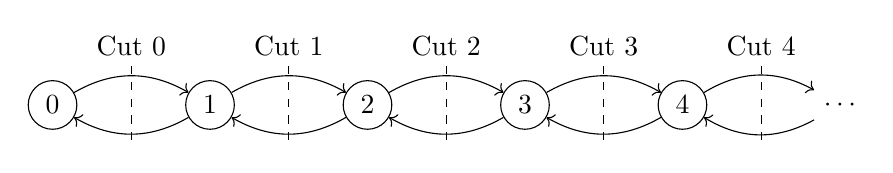
\begin{tikzpicture}
	\foreach \i in {0, 1, 2, 3, 4} {
		\node[draw, circle] (\i) at (2*\i, 0) {$\i$};
	}
	\node (5) at (2*5, 0) {$\cdots$};
	
	\foreach \i/\j in {0/1, 1/2, 2/3, 3/4, 4/5} {
		\draw (\i) edge[->, bend left] (\j);
		\draw (\j) edge[->, bend left] (\i);
		\draw[dashed] ($(\i)!.5!(\j)+(0,.5)$) -- ($(\i)!.5!(\j)-(0,.5)$);
		\node[anchor=south] at ($(\i)!.5!(\j)+(0,.5)$) {Cut $\i$};
	}
	\end{tikzpicture}
	\caption{A birth-and-death process.}
	\label{fig:bd}
\end{figure}

\begin{figure}[ht]
	\centering
	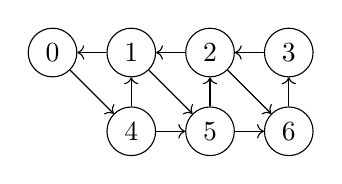
\begin{tikzpicture}
	% nodes
	\foreach \i in {0, 1, ..., 3} {
		\node[state] (\i) at (\i, 0) {$\i$};
	}
	
	\node[state] (bar1) at (1, -1) {$4$};
	\node[state] (bar2) at (2, -1) {$5$};
	\node[state] (bar3) at (3, -1) {$6$};
	
	% edges
	\foreach \i/\j in {0/1, 1/2, 2/3} {
		\draw[->] (\j) -- (\i);
		\draw[->] (\i) -- (bar\j);
	}
	
	\foreach \i/\j in {1/2, 2/3} {
		\draw[->] (bar\i) -- (bar\j);
	}
	
	\foreach \i/\j in {0/1, 1/2, 2/3} {
		\draw[->] (bar\j) -- (\j);
	}
	\end{tikzpicture}
	\caption{A simple formal Markov chain exhibiting a product form relationship between nodes $1$ and $4$, as a result of the cut $(\{0,4\}, \{1,2,3,5,6\})$.}
	\label{fig:jaf-cuts}
\end{figure}

In general, a cut equation~\eqref{eq:cut} as given in \Cref{lem:cut-equations}
is more convenient that the balance equations~\eqref{eq:balance-def}
if the set of nodes~$i$ such that $\pi_i$ appears
on either side of the equation is small.
This set is called the \emph{source} of the corresponding cut,
as it consists of the nodes that are the sources of the edges that cross the cut.

\begin{definition}[Source] \label{def:source}
	Consider a formal Markov chain $G = (V, E)$.
	The source of a cut $(A, B)$ of the graph~$G$
	is the pair $(I, J)$ defined by
	\begin{align} \label{eq:sourced-cut}
		I = \{i \in A: E \cap (\{i\} \times B) \neq \emptyset\},
		\qquad \qquad
		J = \{j \in B: E \cap (\{j\} \times A) \neq \emptyset\}.
	\end{align}
	Equivalently, $(A, B)$ is called an $(I, J)$-sourced cut.
\end{definition}

In \Cref{sec:s-product-form},
we will focus on the special case
where the source sets $I$ and $J$ are both singletons, $I = \{i\}$ and $J = \{j\}$.
We refer to such a cut as a \emph{single-sourced} cut.


\subsection{Joint-ancestor freeness} \label{sec:jaf}

In \Cref{def:jaf} below,
we identify a simpler condition,
called \emph{joint-ancestor freeness},
that we will prove to be necessary and sufficient for
the existence of a cut with a particular source pair
in \Cref{sec:s-product-form-2}.

\begin{definition}[Joint-ancestor freeness] \label{def:jaf}
	Consider a formal Markov chain $G = (V, E)$
	and two disjoint nonempty sets $I, J \subsetneq V$.
	A node~$k \in V$ is a \emph{joint ancestor} of node sets~$I$ and~$J$
	if $k \in A_I(G {\setminus} J) \cap A_J(G {\setminus} I)$,
	i.e., there is both a path from node~$k$ to some node in~$I$ that avoids set~$J$
	and a path from node~$k$ to some node in~$J$ that avoids set~$I$.
	Node sets~$I$ and~$J$ are said to be \emph{joint-ancestor free}
	if $A_I(G {\setminus} J) \cap A_J(G {\setminus} I) = \emptyset$.
	In the special case where $I$ and/or $J$ are singletons,
	we drop the curly brackets in the notation,
	e.g., we write $A_i(G {\setminus} J)$ for $A_{\{i\}}(G {\setminus} J)$.
\end{definition}

To make this definition more concrete,
lets us again consider the birth-and-death process
of \Cref{fig:bd}.
Focusing on $I = \{2\}$ and $J = \{3\}$,
we have $A_2(G {\setminus} 3) = \{0, 1, 2\}$
and $A_3(G {\setminus} 2) = \{3, 4, 5, \ldots\}$,
so that nodes~2 and~3 are joint-ancestor free.
To see why $A_2(G {\setminus} 3) = \{0, 1, 2\}$,
it suffices to observe that
the subgraph $G {\setminus} 3$ consists of two strongly connected components:
$\{0, 1, 2\}$ and $\{4, 5, 6, \ldots\}$.
Anticipating over \Cref{prop:jaf-cuts-1} below,
we observe that 
$(A_2(G {\setminus} 3), A_3(G {\setminus} 2))
= (\{0, 1, 2\}, \{3, 4, 5, \ldots\})$
is exactly Cut~2 in \Cref{fig:bd}.
Similarly, $I = \{1\}$ and $J = \{2, 4\}$
are joint-ancestor free because
$A_1(G {\setminus} \{2, 4\}) = \{0, 1\}$
and $A_{\{2, 4\}}(G {\setminus} 1) = \{2, 3, 4, \ldots\}$.
On the contrary, nodes~1 and~3 are not joint-ancestor free
because $A_1(G {\setminus} 3) = \{0, 1, 2\}$
and $A_3(G {\setminus} 1) = \{2, 3, 4, \ldots\}$
have non-empty intersection $\{2\}$.

The \textsc{MutuallyAvoidingAncestors} procedure
in \Cref{algo:jaf}
returns the joint-ancestor sets $A_I(G {\setminus} J)$ and $A_J(G {\setminus} I)$
in time $O(|E|)$ in a finite graph $G$,
by calling the \textsc{Ancestors} procedure
from \Cref{algo:ancestors}.
\textsc{MutuallyAvoidingAncestors} can be used to test
if two node sets are joint-ancestor free.

\begin{algorithm}[htb]
	\caption{Returns the mutually-avoiding ancestors of two node sets}
	\label{algo:jaf}
	\begin{algorithmic}[1]
		\Procedure{MutuallyAvoidingAncestors}{finite directed graph $G = (V, E)$, disjoint non\-empty sets~$I, J \subseteq V$}
		$\to$ ancestor sets $A_I(G {\setminus} J), A_J(G {\setminus} I)$
		\State $A_I \gets$ \Call{Ancestors}{$I$, $G {\setminus} J$}
		\State $A_J \gets$ \Call{Ancestors}{$J$, $G {\setminus} I$}
		\State \Return $A_I, A_J$
		\EndProcedure
	\end{algorithmic}
\end{algorithm}





\section{S-product-form, cuts, and joint-ancestor freeness}
\label{sec:s-product-form}

In this section, we focus on the S-product-form relationship
introduced in \Cref{sec:product-form-def}.
\Cref{theo:s-product-form}, the main result of this section,
is stated in \Cref{sec:s-product-form-main}
and illustrated on toy examples in \Cref{sec:s-product-form-examples}.
The proof of \Cref{theo:s-product-form}
relies on intermediary results shown in
\Cref{sec:s-product-form-1,sec:s-product-form-2,sec:s-product-form-3}.
Higher-order product-form relationships,
such as PS-product-form,
will be considered in \Cref{sec:higher-levels}.

\subsection{Main theorem} \label{sec:s-product-form-main}

\Cref{theo:s-product-form} below is our first main contribution:
it gives simple necessary and sufficient conditions
under which two nodes are in an S-product-form relationship.
This result relies on the two graph-based notions introduced earlier,
namely, cuts with a given source node (\Cref{sec:cuts})
and joint-ancestor freeness (\Cref{sec:jaf}).
The rest of \Cref{sec:s-product-form} will give further insights into this result.

\begin{theorem} \label{theo:s-product-form}
	Consider a formal Markov chain~$G = (V, E)$
	and let~$i, j \in V$.
	The following statements are equivalent:
	\begin{enumerate}[(i)]
		\item \label{item:S-product-form-1}
		Nodes~$i$ and~$j$ are in an S-product-form relationship.
		\item \label{item:S-product-form-2}
		There is an $i, j$-sourced cut.
		\item \label{item:S-product-form-3}
		Nodes~$i$ and $j$ are joint-ancestor free.
	\end{enumerate}
	If these statements are true, then
	the S-product-form between nodes~$i$ and~$j$ has factors
	\begin{align}
		\label{eq:first-level-product-form}
		f_{i, j} = \sum_{\substack{k \in A_j(G {\setminus} i): \\ (i, k) \in E}} q_{i, k}
		\quad \text{and} \quad
		f_{j, i} = \sum_{\substack{k \in A_i(G {\setminus} j): \\ (j, k) \in E}} q_{j, k}.
	\end{align}
\end{theorem}

\begin{proof}
	The implication \eqref{item:S-product-form-2} $\implies$ \eqref{item:S-product-form-1}
	is a classical result that will be recalled
	in \Cref{lem:cut-implies-product-form} in \Cref{sec:s-product-form-1}.
	The equivalence \eqref{item:S-product-form-2} $\iff$ \eqref{item:S-product-form-3}
	will be shown in \Cref{prop:jaf-cuts-1} in \Cref{sec:s-product-form-2}.
	The implication \eqref{item:S-product-form-1} $\implies$ \eqref{item:S-product-form-3}
	will be shown in \Cref{theo:no-product-form} in \Cref{sec:s-product-form-3}.
	Lastly, Equation~\eqref{eq:first-level-product-form} follows for instance
	by combining \Cref{lem:cut-implies-product-form} and \Cref{prop:jaf-cuts-1}.
\end{proof}

The equivalence between conditions
\eqref{item:S-product-form-1} and \eqref{item:S-product-form-2}
is reminiscent of classical sufficient conditions
on the existence of a product-form relationship,
except that the focus is now on the transition graph
rather than on the transition rates.
Now, the equivalence between conditions
\eqref{item:S-product-form-2} and \eqref{item:S-product-form-3}
can be intuitively understood as follows.
If two nodes $i, j \in V$ are joint-ancestor free,
meaning that  $A_i(G {\setminus} j) \cap A_j(G {\setminus} i) = \emptyset$,
then one can verify that $(A_i(G {\setminus} j), A_j(G {\setminus} j))$
forms a cut and that its source nodes are $i$ and $j$.
On the contrary, if $i$ and $j$ are not joint-ancestor free,
there exists $k \in V {\setminus} \{i, j\}$
such that there are two paths $P(k \to i {\setminus} j)$
and $P(k \to j {\setminus} i)$.
The existence of these two paths
precludes any cut $(A, B)$
from having source $i, j$.
Indeed, assuming for example that $i, k \in A$ and $j \in B$,
the path $P(k \to j {\setminus} i)$
needs to go from part~$A$ (containing~$k$)
to part~$B$ (containing~$j$),
and it cannot do so via node~$i$
since this is an $i$-avoiding path.
Therefore, the source of part~$A$ cannot be reduced to node~$i$.

Thanks to \Cref{theo:s-product-form},
we can directly apply procedure \textsc{MutuallyAvoidingAncestors} from \Cref{algo:jaf}
to verify if two nodes~$i$ and~$j$ are in an S-product-form relationship
and, if yes, compute the corresponding factors,
all with time complexity $O(|E|)$.
This is far more efficient than directly testing each cut in the graph to see if its sources are $i$ and $j$:
there are $2^{|V|}$ such cuts, each of which would take $|E|$ time to check.
Testing the S-product-form relationship of all pairs of nodes in the graph
can be done in time $O(|V|^2 |E|)$
(also see \Cref{sec:cut-graph}).



\subsection{Illustrative examples} \label{sec:s-product-form-examples}

Before we prove the intermediary results
that appear in the proof of \Cref{theo:s-product-form},
let us illustrate this connection between single-sourced cuts, joint-ancestor freeness, and product-form relationships with a few toy examples, shown in \Cref{fig:bd,fig:illustrative-examples}.
We first revisit the birth-and-death process
already discussed in \Cref{sec:cuts,sec:jaf}.
For a more sophisticated example involving S-product-form,
please see \Cref{sec:msj-example}.

\begin{example}[Birth-and-death process]
	Consider a formal Markov chain $G = (V, E)$ with
	$V = \{0, 1, 2, \ldots\}$ and $E = \bigcup_{i \in V} \{(i, i+1), (i+1, i)\}$,
	as in \Cref{fig:bd}.
	For each $i \in V$,
	nodes~$i$ and~$i+1$ are in an S-product-form relationship
	through the $i, i+1$-sourced cut formed by
	$A_i(G {\setminus} i+1) = \{1, 2, \ldots, i\}$
	and $A_{i+1}(G {\setminus} i) = \{i+1, i+2, \ldots\}$.
	However, for each $i, j \in V$
	such that $i \le j - 2$,
	nodes~$i$ and~$j$ are not in an S-product-form relationship
	because $A_i(G {\setminus} j) = \{0, 1, 2, \ldots, j-1\}$
	and $A_j(G {\setminus} i) = \{i+1, i+2, \ldots, n\}$
	intersect at
	$A_i(G {\setminus} j) \cap A_j(G {\setminus} i)
	= \{i+1, i+2, \ldots, j-1\}$.
\end{example}

\begin{figure}[htb]
	\begin{subfigure}{.3\linewidth}
		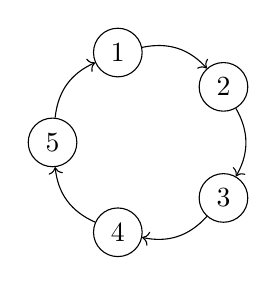
\begin{tikzpicture}
		\foreach \a in {1, 2, ..., 5} {
			\node[state] (\a) at (180-\a*360/5: 1.2cm) {\a};
		}
		\foreach \a/\b in {1/2, 2/3, 3/4, 4/5, 5/1} {
			\draw (\a) edge[->, bend left] (\b);
		}
		\end{tikzpicture}
		\caption{One-way cycle}
		\label{fig:one-way-cycle}
	\end{subfigure}
	\hfill
	\begin{subfigure}{.3\linewidth}
		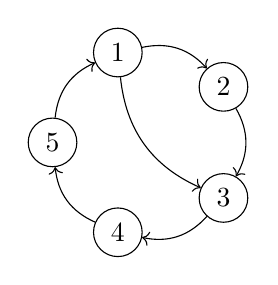
\begin{tikzpicture}
		\foreach \a in {1, 2, ..., 5} {
			\node[state] (\a) at (180-\a*360/5: 1.2cm) {\a};
		}
		\foreach \a/\b in {1/2, 2/3, 3/4, 4/5, 5/1} {
			\draw (\a) edge[->, bend left] (\b);
		}
		\draw (1) edge[->, bend right] (3);
		\end{tikzpicture}
		\caption{One-way cycle with an additional edge}
		\label{fig:one-way-cycle-with-edge}
	\end{subfigure}
	\hfill
	\begin{subfigure}{.3\linewidth}
		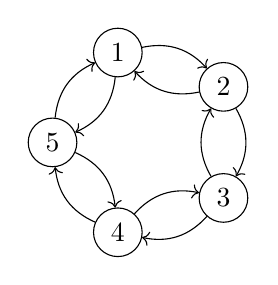
\begin{tikzpicture}
		\foreach \a in {1, 2, ..., 5} {
			\node[state] (\a) at (180-\a*360/5: 1.2cm) {\a};
		}
		\foreach \a/\b in {1/2, 2/3, 3/4, 4/5, 5/1} {
			\draw (\a) edge[->, bend left] (\b);
			\draw (\b) edge[->, bend left] (\a);
		}
		\end{tikzpicture}
		\caption{Two-way cycle}
		\label{fig:two-way-cycle}
	\end{subfigure}
	\caption{Illustrative examples of S-product-form relationships.}
	\label{fig:illustrative-examples}
\end{figure}

\begin{example}[One-way cycle] \label{ex:one-way-cycle}
	Consider a formal Markov chain $G = (V, E)$ with
	$V = \{1, 2, \ldots, n\}$ for some $n \ge 3$
	and $E = \{(i, i+1) | i \in V\} \cup E'$,
	where $E' \subseteq \{(i, i) | i \in V\}$,
	with the convention that nodes are numbered modulo~$n$.
	For instance, \Cref{fig:one-way-cycle}.
	For each $i, j \in V$, say with $i < j$,
	the sets
	$A_i(G {\setminus} j)= \{j+1, j+2, \ldots, n, 1, 2, \ldots, i\}$
	and $A_j(G {\setminus} i) = \{i+1, i+2, \ldots, j\}$
	are disjoint and therefore form an $i, j$-sourced cut.
	\Cref{theo:s-product-form} implies that
	nodes~$i$ and~$j$ are in an S-product-form relationship with
	$f_{i, j} = q_{i, i+1}$ and $f_{j, i} = q_{j, j+1}$.
	Equivalently, we can check visually
	that there is no node from which there is a directed path
	to node~$i$ without visiting node~$j$ and vice versa.
	This example shows in particular that an $i, j$-sourced cut may exist
	even if there is neither an edge~$(i, j)$ nor an edge~$(j, i)$.
\end{example}

\begin{example}[One-way cycle with an additional edge]
	Consider the same directed cycle,
	but with an additional edge
	from node~$1$ to some node~$k \in \{3, 4, \ldots, n\}$.
	For instance, \Cref{fig:one-way-cycle-with-edge}.
	For each $i \in \{2, 3, \ldots, k - 1\}$
	and $j \in \{k, k + 2, \ldots, n\}$,
	nodes~$i$ and~$j$ are no longer joint-ancestor free because
	$1 \in A_i(G {\setminus} j) \cap A_j(G {\setminus} i)$.
	Indeed,
	$1 \to 2 \to 3 \to \cdots \to i$
	is a $P(1 \to i {\setminus} j)$ path
	and
	$1 \to k \to k + 1 \to \dots \to j$
	is a $P(1 \to j {\setminus} i)$ path.
	Therefore, nodes~$i$ and~$j$ are no longer
	in an S-product-form relationship.
\end{example}

\begin{example}[Two-way cycle]
	Lastly, consider a directed graph $G = (V, E)$ with
	$V = \{1, 2, \ldots, n\}$ for some $n \ge 3$
	and $E = \bigcup_{i \in V} \{(i, i+1), (i+1, i)\}$,
	again with the convention that nodes are numbered modulo~$n$.
	For instance, \Cref{fig:two-way-cycle}.
	For each $i, j \in V$, the sets
	$A_i(G {\setminus} j) = V {\setminus} \{j\}$
	and $A_j(G {\setminus} i) = V {\setminus} \{i\}$
	have nonempty intersection
	$A_i(G {\setminus} j) \cap A_j(G {\setminus} i) = V {\setminus} \{i, j\}$.
	Hence, there are no S-product-form relationships in this graph.
\end{example}





\subsection{The existence of a single-sourced cut implies S-product-form} \label{sec:s-product-form-1}

\Cref{lem:cut-implies-product-form} below shows the implication
\eqref{item:S-product-form-2} $\implies$ \eqref{item:S-product-form-1}
from \Cref{theo:s-product-form}.
This result is recalled for completeness,
but it follows directly by combining
the definition of a sourced cut (\Cref{def:source})
with \Cref{lem:cut-equations}.

\begin{lemma}
	\label{lem:cut-implies-product-form}
	Consider a formal Markov chain~$G = (V, E)$
	and two nodes~$i, j \in V$.
	If there is an $i, j$-sourced cut in the graph~$G$,
	then these nodes are in an S-product-form relationship~\eqref{eq:product-form},
	with factors as given in~\eqref{eq:first-level-product-form}.
\end{lemma}



\subsection{The existence of a single-sourced cut is equivalent to joint-ancestor freeness} \label{sec:s-product-form-2}

We now prove
the equivalence
\eqref{item:S-product-form-2} $\iff$ \eqref{item:S-product-form-3}
from \Cref{theo:s-product-form},
that is, joint-ancestor freeness
is necessary and sufficient
for the existence of a cut with a particular source pair.
We show that this equivalence holds
both when the source pair is a pair $i, j$ of nodes
(\Cref{prop:jaf-cuts-1})
and more generally for any pair $I, J$ of source sets
(\Cref{prop:jaf-cuts-2}).
Cuts where the source pair is a general pair of source sets $I, J$ give rise to
higher-level cuts, as we show and discuss in \Cref{sec:higher-levels}.

\begin{proposition} \label{prop:jaf-cuts-1}
	Consider a formal Markov chain $G = (V, E)$
	and let $i, j \in V$.
	Nodes~$i$ and~$j$ are joint-ancestor free
	if and only if
	there exists an $i, j$-sourced cut.
	In this case, the only $i, j$-sourced cut is
	$(A_i(G {\setminus} j), A_j(G {\setminus} i))$.
\end{proposition}

\Cref{prop:jaf-cuts-1} is a special case of \Cref{prop:jaf-cuts-2},
which is stated and proved later in this section.
To illustrate the intuition behind \Cref{prop:jaf-cuts-1},
again consider the toy example of \Cref{fig:jaf-cuts}.
Nodes $1$ and $4$ are joint-ancestor free
because $A_1(G {\setminus} 4) = \{1, 2, 3, 5, 6\}$
and $A_4(G {\setminus} 1) = \{0, 4\}$ are disjoint
and therefore form a $1, 4$-sourced cut.
In contrast, nodes~$1$ and~$2$ are not joint-ancestor free
because $A_1(G {\setminus} 2) = \{0, 1, 4\}$
and $A_2(G {\setminus} 1) = \{2, 3, 4, 5, 6\}$
intersect at node~$4$.
Any cut $(A, B)$ such that $1 \in A$ and $2 \in B$
has to be crossed by an edge from a path $P(4 \to 2 {\setminus} 1)$
(if $4 \in A$)
or from a path $P(4 \to 1 {\setminus} 2)$
(if $4 \in B$),
which makes it impossible to build a cut
whose sources are restricted to nodes~$1$ and~$2$.
This intuition is formalized
in Statement~\eqref{prop:ancestors-2}
of \Cref{lem:jaf-cuts} below.
\Cref{prop:jaf-cuts-1} implies in particular that
an $i, j$-sourced cut is unique when it exists,
hence we can say \emph{the} $i, j$-sourced cut.

For \Cref{prop:jaf-cuts-2} below, the situation is slightly more complicated.
When considering
joint-ancestor free sets $I, J$ containing more than one node,
cuts may not be unique, and may not have the entire sets $I, J$ as sources.
Nonetheless, there is still a bidirectional relationship between mutually-avoiding ancestor sets
and cut-source sets.

\begin{proposition} \label{prop:jaf-cuts-2}
	Consider a formal Markov chain $G = (V, E)$
	and two disjoint non\-empty sets $I, J \subseteq V$.
	We have the following:
	\begin{enumerate}[(i)]
		\item \label{prop:ancestors-4}
		If $I$ and $J$ are joint-ancestor free,
		then the cut $(A_I(G {\setminus} J), A_J(G {\setminus} I))$
		is an $(\underline{I}, \underline{J})$-sourced cut, for some non-empty sets $\underline{I} \subseteq I$ and $\underline{J} \subseteq J$.
		\item \label{prop:ancestors-5}
		If $(A_I(G {\setminus} J), A_J(G {\setminus} I))$ is a cut and has sources $(I, J)$, then it is the unique cut with sources ($I$, $J$).
		\item \label{prop:ancestors-3}
		If $I$ and $J$ are not joint-ancestor free,
		then there is no $(I, J)$-sourced cut.
	\end{enumerate}
\end{proposition}

Again considering the example of \Cref{fig:jaf-cuts},
let $I = \{1, 4\}$ and $J = \{2, 5\}$.
The ancestor sets
$A_I(G {\setminus} J) = \{0, 1, 4\}$
and $A_J(G {\setminus} I) = \{2, 3, 5, 6\}$
are disjoint,
and we can verify that they form an
$(\underline{I}, \underline{J})$ sourced-cut
with $\underline{I} = \{1, 4\} = I$
and $\underline{J} = \{2\} \subsetneq J$.
%
For a negative example, node sets
$I' = \{1\}$ and $J = \{2, 5\}$ are not joint-ancestor free
because $A_{I'}(G {\setminus} J) = \{0, 1, 4\}$
and $A_{J}(G {\setminus} I') = \{2, 3, 4, 5, 6\}$
intersect at node~$4$.
Correspondingly, one can verify that there is no $(I', J)$-sourced cut in the graph.

Before proving \Cref{prop:jaf-cuts-1,prop:jaf-cuts-2},
we prove the following intermediary lemma,
which will also be instrumental for later results.

\begin{lemma} \label{lem:jaf-cuts}
	Consider a formal Markov chain $G = (V, E)$
	and two disjoint non\empty sets $I, J \subsetneq V$.
	We have the following:
	\begin{enumerate}[(i)]
		\item \label{prop:ancestors-1}
		$A_I(G {\setminus} J) \cup A_J(G {\setminus} I) = V$.
		\item \label{prop:ancestors-2}
		If $(A, B)$ is an $(I, J)$-sourced cut,
		then $A_I(G {\setminus} J) \subseteq A$
		and $A_J(G {\setminus} I) \subseteq B$.
	\end{enumerate}
\end{lemma}
\begin{proof}[Proof of \Cref{lem:jaf-cuts}]
	Let us first prove \Cref{lem:jaf-cuts}\eqref{prop:ancestors-1}.
	Let $k \in V$.
	Since $G$ is strongly connected
	and $I$ is nonempty,
	there is a directed path
	$v_1, v_2, \ldots, v_n$ in $G$,
	with $n \ge 1$,
	such that $v_1 = k$ and $v_n \in I$.
	Let $p = \min\{q \in \{1, 2, \ldots, n\} | k_q \in I \cup J\}$.
	Then $k \in A_I(G {\setminus} J)$ if $k_p \in I$
	and $k \in A_J(G {\setminus} I)$ if $k_p \in J$.
	Hence, $k \in A_I(G {\setminus} J) \cup A_J(G {\setminus} I)$
	for each $k \in V$, which implies that $V = A_I(G {\setminus} J) \cup A_J(G {\setminus} I)$.
	
	We now prove \Cref{lem:jaf-cuts}\eqref{prop:ancestors-2}.
	Assume that $(A, B)$ is an $(I, J)$-sourced cut
	and let $k \in A_I(G {\setminus} J)$:
	there is a directed path $v_1, v_2, \ldots, v_n$
	such that $v_1 = k$, $v_n \in I$,
	and $v_p \notin J$ for each $p \in \{1, 2, \ldots, n\}$.
	Our goal is to prove that $k \in A$.
	If $n = 1$, we have directly $k \in I \subseteq A$.
	Now consider the case where $n \ge 2$.
	Assume for the sake of contradiction that $k \notin A$,
	that is, $k \in B$,
	so that $v_1 = k \in B$ and $v_n \in A$.
	Then we can define
	$p = \max\{q \in \{1, 2, \ldots, n-1\} | v_q \in B\}$,
	and we have $(v_p, v_{p+1}) \in E \cap (B \times A)$.
	We also know by construction of the path that $k_p \notin J$.
	This contradicts our assumption that $J$ is the second source of the cut~$(A, B)$.
	Hence, $k \in A$.
\end{proof}

\begin{proof}[Proof of \Cref{prop:jaf-cuts-1,prop:jaf-cuts-2}]
	\Cref{prop:jaf-cuts-1} is a special case of \Cref{prop:jaf-cuts-2}
	because the only nonempty subset of a singleton is the singleton itself.
	Therefore, in the remainder, we focus on proving \Cref{prop:jaf-cuts-2}.
	
	Let us first prove \Cref{prop:jaf-cuts-2}\eqref{prop:ancestors-4}.
	Assume that $I$ and $J$ are joint-ancestor free,
	that is, $A_I(G {\setminus} J) \cap A_J(G {\setminus} I) = \emptyset$.
	Combining this assumption with
	\Cref{lem:jaf-cuts}\eqref{prop:ancestors-1}
	shows that $(A_I(G {\setminus} J), A_J(G {\setminus} I))$
	is a cut.
	Assume for the sake of contradiction that
	the source $(\underline{I}, \underline{J})$
	of the cut $(A_I(G {\setminus} J), A_J(G {\setminus} I))$
	does not satisfy $\underline{I} \subseteq I$
	and $\underline{J} \subseteq J$.
	Specifically, suppose
	there exists $(k, \ell) \in E \cap (A_I(G {\setminus} J) \times A_J(G {\setminus} I))$
	such that $k \notin I$.
	Since $\ell \in A_J(G {\setminus} I)$,
	there exists a directed path
	$v_1, v_2, \ldots, v_n$, with $n \ge 1$,
	such that $v_1 = \ell$, $v_n = j \in J$,
	and $v_p \notin I$ for each $p \in \{1, 2, \ldots, n\}$.
	Since we assumed $k \notin I$,
	it follows that $k, v_1, v_2, \ldots, v_n$ is a directed path
	from $k$ to~$j$ in $G {\setminus} I$,
	hence $k \in A_J(G {\setminus} I)$,
	which is impossible since we assumed $k \in A_I(G {\setminus} J)$
	and $A_I(G {\setminus} J) \cap A_J(G {\setminus} I) = \emptyset$.
	
	Next, we prove \Cref{prop:jaf-cuts-2}\eqref{prop:ancestors-5}.
	By \Cref{lem:jaf-cuts}\eqref{prop:ancestors-2}, any cut $(A, B)$ with source $(I, J)$ is such that
	$A_I(G {\setminus} J) \subseteq A$
	and $A_J(G {\setminus} I) \subseteq B$.
	But we assumed $(A_I(G {\setminus} J), A_J(G {\setminus} I))$ forms a cut,
	and no nodes can be outside of the cut.
	Thus, $A_I(G {\setminus} J) = A$ and $A_J(G {\setminus} I) = B$.
	
	Lastly, we prove \Cref{prop:jaf-cuts-2}\eqref{prop:ancestors-3}.
	Assume that $I$ and $J$ are not joint-ancestor free,
	i.e., $A_I(G {\setminus} J) \cap A_J(G {\setminus} I) \neq \emptyset$.
	Assume for the sake of contradiction that
	there is a cut $(A, B)$ with source $(I, J)$.
	\Cref{lem:jaf-cuts}\eqref{prop:ancestors-2} implies that
	$A_I(G {\setminus} J) \subseteq A$
	and $A_J(G {\setminus} I) \subseteq B$,
	which in turn implies that
	$A \cap B \supseteq A_I(G {\setminus} J) \cap A_J(G {\setminus} I) \neq \emptyset$.
	This contradicts our assumption that $(A, B)$ is a cut.
\end{proof}



\subsection{S-product-form implies joint-ancestor freeness} \label{sec:s-product-form-3}

Our last step in the proof of \Cref{theo:s-product-form}
is to show the implication
\eqref{item:S-product-form-1} $\implies$ \eqref{item:S-product-form-3},
that is,
S-product-form relationship implies joint-ancestor freeness.
We have shown so far that statements
\eqref{item:S-product-form-2} and \eqref{item:S-product-form-3}
are equivalent to each other,
and that they imply \eqref{item:S-product-form-1}.
In other words,
we proved that if a $i,j$-sourced cut exists, or equivalently if nodes~$i$ and $j$ have no joint ancestor, then an S-product-form relationship between $i$ and $j$ exists. Specifically, a product-form relationship exists where $f_{i,j}$ depends only on transition rates along edges whose source is $i$, and $f_{j,i}$ depends only on transition rates along edges whose source is $j$.

\Cref{theo:no-product-form} below proves this condition is necessary.
The intuition behind the proof is as follows.
If an $i,j$-sourced cut does not exist, then by \Cref{prop:jaf-cuts-1} there exist nodes 
which are ancestors of both $i$ and $j$, i.e., $A_i(G\setminus j) \cap A_j(G {\setminus} i)$ is nonempty. In particular, there must exist a node $k$ which is an ancestor of both nodes $i$ and $j$ via disjoint paths.
If such a node $k$ exists, we show that the ratio $\frac{\pi_i}{\pi_j}$ depends on edge weights $q_{k, k'}$ with source $k$.
This violates the definition of S-product-form given in \Cref{sec:product-form-def}, so \Cref{theo:no-product-form} shows that a joint ancestor implies no S-product-form, or equivalently that S-product-form implies no joint ancestor.

\begin{theorem}
	\label{theo:no-product-form}
	Consider a formal Markov chain $G = (V, E)$
	and let $i, j \in V$.
	Suppose nodes~$i$ and~$j$ are not joint-ancestor free,
	i.e., $A_i(G {\setminus} j) \cap A_j(G {\setminus} i) \neq \emptyset$.
	
	Then there exists a node $k \in A_i(G {\setminus} j) \cap A_j(G {\setminus} i)$ such that the stationary probability ratio $\frac{\pi_i}{\pi_j}$ depends on at least one of edge weights emerging from $k$.
\end{theorem}

\begin{proof}
	We will choose $k$ to be a node in $A_i(G {\setminus} j) \cap A_j(G {\setminus} i)$ such that $k$ is an ancestor of both nodes $i$ and $j$ via disjoint paths.
	To see why such a node must exist, consider an arbitrary node $k'$ in $A_i(G {\setminus} j) \cap A_j(G {\setminus} i)$. From any such node, there exist paths from $k'$ to $i$ and $k'$ to $j$.
	Consider the shortest such paths. Either these paths are disjoint,
	or there is a node $k''$ which is a joint ancestor of $i$ and $j$ via shorter paths than $k'$.
	Over all nodes in $A_i(G {\setminus} j) \cap A_j(G {\setminus} i)$,
	let $k$ be the node that is the ancestor of $i$ via the shortest path length, choosing arbitrarily in case of a tie.
	By the above argument, the shortest paths from $k$ to $i$ and from $k$ to $j$ must be disjoint.
	
	Let $a$ be the shortest path from $k$ to $i$, $a := k, a_2, a_3, \ldots, i$.
	Let $b$ be the shortest path from $k$ to $j$, $b := k, b_2, b_3, \ldots, j$. As shown above, $a$ and $b$ share no nodes except node $k$.
	
	Consider the subchain,
	with node set $U = \{i, j, k\}$,
	obtained by looking at the subsequence of states
	visited by the original Markov chain $G = (V, E)$
	inside the set~$U$.
	This subchain satisfies the Markov property,
	and for each $u, v \in U$
	we let $p_{u, v}$ denote
	its transition probability
	from state~$u$ to state~$v$;
	these are functions of the original Markov chain's
	transition rates~$q_{i, j}$ for $i, j \in V$.
	Critically, letting $\pi_i$, $\pi_j$, and $\pi_k$
	denote the stationary probabilities for states $i$, $j,$ and $k$
	in the original Markov chain,
	as defined by~\eqref{eq:balance-def},
	we can verify that
	$\frac{\pi_i}{\pi_i + \pi_j + \pi_k}$,
	$\frac{\pi_j}{\pi_i + \pi_j + \pi_k}$,
	and $\frac{\pi_k}{\pi_i + \pi_j + \pi_k}$
	form the stationary distribution of the subchain.
	Using this definition,
	we will quantify the relative state probabilities $\pi_i$ and $\pi_j$ in terms of the subchain transition probabilities $p_{u, v}$ for $u,v \in U$.
	
	Using the balance equations for the subchain, we obtain successively:
	\begin{align}
		\label{eq:subchain-1}
		\pi_k &= p_{ik} \pi_i + p_{jk} \pi_j + p_{kk} \pi_k, \\
		\label{eq:subchain-2}
		\pi_k &= \frac{p_{ik} \pi_i + p_{jk} \pi_j}{1-p_{kk}}, \\
		\label{eq:subchain-3}
		\pi_i &= p_{ii} \pi_i + p_{ji} \pi_j + p_{ki} \pi_k, \\
		\label{eq:subchain-4}
		\pi_i &= p_{ii} \pi_i + p_{ji} \pi_j + p_{ki} \frac{p_{ik} \pi_i + p_{jk} \pi_j}{1-p_{kk}}, \\
		\label{eq:subchain-5}
		\pi_i \left(1 - p_{ii} - \frac{p_{ik} p_{ki}}{1-p_{kk}} \right)
		&= \pi_j \left(p_{ji} + \frac{p_{jk} p_{ki}}{1-p_{kk}}\right), \\
		\label{eq:subchain-6}
		\pi_i \left(p_{ij} + p_{ik} - \frac{p_{ik} p_{ki}}{p_{ki} + p_{kj}} \right)
		&= \pi_j \left(p_{ji} + \frac{p_{jk} p_{ki}}{p_{ki} + p_{kj}}\right), \\
		\label{eq:subchain-7}
		\pi_i \left(p_{ij} + p_{ik} \frac{p_{kj}}{p_{ki} + p_{kj}} \right)
		&= \pi_j \left(p_{ji} + p_{jk} \frac{p_{ki}}{p_{ki} + p_{kj}}\right).
	\end{align}
	Equations~\eqref{eq:subchain-1} and~\eqref{eq:subchain-3}
	are the balance equations of the subchain
	for states~$k$ and~$i$.
	Equation~\eqref{eq:subchain-2} follows
	by solving~\eqref{eq:subchain-1} with respect to~$\pi_k$,
	and once injected into~\eqref{eq:subchain-3}
	it yields~\eqref{eq:subchain-4}.
	Equation~\eqref{eq:subchain-5}
	follows by rearranging~\eqref{eq:subchain-4},
	and becomes~\eqref{eq:subchain-6} after injecting
	$p_{ii} + p_{ij} + p_{ik} = 1$.
	Equation~\eqref{eq:subchain-7} then follows
	by rearraging~\eqref{eq:subchain-6}.
	
	Equation~\eqref{eq:subchain-7} shows that,
	if we change $\frac{p_{ki}}{p_{ki} + p_{kj}}$
	while holding $p_{ij}, p_{ik}, p_{ji}, p_{jk}$ constant,
	then the relative probabilities of $\pi_i$ and $\pi_j$ will change.
	Therefore, to conclude, it suffices to show that, by only changing $q_{k,a_2}$ and $q_{k,b_2}$, $\frac{p_{ki}}{p_{ki} + p_{kj}}$ can be changed while holding $p_{ij}, p_{ik}, p_{ji}, p_{jk}$ constant.
	Specifically, in the remainder of the proof, we show that if certain free variables $q_{c, d}$ in the graph are fixed to specific values, and $q_{k,a_2}$ and $q_{k,b_2}$ are left free to vary,
	then $\frac{p_{ki}}{p_{ki} + p_{kj}}$ can still vary.
	This implies that $\frac{p_{ki}}{p_{ki} + p_{kj}}$ depends on $q_{k,a_2}$ and $q_{k,b_2}$,
	as desired.
	We can immediately note that $q_{k,a_2}$ and $q_{k,b_2}$ have no effect on $p_{ij}, p_{ik}, p_{ji},$ or $p_{jk}$,
	as $(k, a_2)$ and $(k, b_2)$ originate at $k$, and therefore cannot be visited on $k$-avoiding paths from $i$ to $j$ or any of the other pairs listed.
	
	Recall that we label the nodes within paths $a$ and $b$ as $a_1, a_2, \ldots$ and $b_1, b_2, \ldots$,
	with $a_1 = b_1 = k$. Let $|a|, |b|$ be the number of edges within each path. There are $|a|+1$ and $|b|+1$ nodes in the paths, and $a_{|a|+1} = i$, and $b_{|b|+1} = j$.
	All other nodes within $a$ and $b$ are disjoint, and are neither $i, j,$ nor $k$.
	
	Let us fix all edge weights $q$ whose source nodes are within path $a$, other than nodes $k$ and $i$.
	We will show that even with these edge weights fixed, changing $q_{k,a_2}$ and $q_{k,b_2}$
	still affects $\frac{p_{ki}}{p_{ki} + p_{kj}}$.
	
	Let $\epsilon > 0$ be a constant to be specified later,
	and let $\Delta(v)$ be the degree of node~$v$.
	Let us specify the edge weights for edges whose source node is within $a$ as follows:
	\begin{align*}
		q_{a_\ell,a_{\ell+1}} &:= 1-\epsilon,
		\quad \forall \ell, 2 \le \ell \le |a|, \\
		q_{a_\ell, a'} &:= \frac{\epsilon}{\Delta(a_i)-1},
		\quad \forall a' \neq a_{\ell+1}, (a_\ell, a') \in E.
	\end{align*}
	Note that we have fixed the edge weight for all edges whose source node is within $a$,
	except for $a_1 = k$ and $a_{|a|+1} = i$.
	We fix the edge weights for nodes whose source vertex is within $b$ in the same manner.
	Let us also fix all edge weights whose source node is $k$, other than $q_{k,a_2}$ and $q_{k,b_2}$,
	to be $\frac{\epsilon}{\Delta(k)-1}$.
	
	Now, we consider two extreme configurations: 
	\begin{enumerate}[(a)]
		\item The $a$-emphasizing configuration: $q_{k,a_2} = 1 - \epsilon$, and $q_{k,b_2} = \frac{\epsilon}{\Delta(k)-1}$.
		\label{item:a-conf}
		\item The $b$-emphasizing configuration: $q_{k,b_2} = 1 - \epsilon$, and $q_{k,a_2} = \frac{\epsilon}{\Delta(k)-1}$.
		\label{item:b-conf}
	\end{enumerate}
	Let us bound $p_{ki}$ and $p_{kj}$ in each configuration.
	In Configuration~\ref{item:a-conf},
	the system may move from $k$ to $i$ via traversing path $a$.
	Each edge weight in this path has probability $(1-\epsilon)$, so
	$p_{ki}^{(a)} \ge (1-\epsilon)^{|a|}$.
	A similar lower bound holds in Configuration~\ref{item:b-conf}:
	$p_{kj}^{(b)} \ge (1-\epsilon)^{|b|}$.
	
	Let us specify $\epsilon = 3 \max(|a|, |b|)$.
	Note that for all $x \ge 1$,
	$(1-\frac{1}{3x})^x \in [2/3, e^{-1/3})$.
	As a result,
	$p_{ki}^{(a)} \ge 2/3$ and $p_{kj}^{(b)} \ge 2/3$,
	which yields
	\begin{align*}
		\frac{p_{ki}^{(a)}}{p_{ki}^{(a)} + p_{kj}^{(a)}} &\ge 2/3, &
		\frac{p_{ki}^{(b)}}{p_{ki}^{(b)} + p_{kj}^{(b)}} &\le 1/3.
	\end{align*}
	Between Configurations~\ref{item:a-conf} and~\ref{item:b-conf},
	only $q_{k,a_2}$ and $q_{k,b_2}$ changed, and yet $\frac{p_{ki}}{p_{ki} + p_{kj}}$ changed.
	Thus, between Configurations~\ref{item:a-conf} and~\ref{item:b-conf},
	the relative probability $\frac{\pi_i}{\pi_j}$ changes.
	As a result, $\frac{\pi_i}{\pi_j}$ depends on at least one of $q_{k,a_2}$ and $q_{k,b_2}$,
	both with partially-fixed weights and with all weights as free variables.
\end{proof}






\section{Cut graph and higher-level cuts} \label{sec:higher-levels}

In this section, we explore product-form relationships beyond the S-product-form
which was the focus of \Cref{sec:s-product-form}.
In \Cref{sec:cut-graph}, we define the cut graph, which is an undirected graph whose edges represent S-product-form relationships between nodes.
Based on this definition, in \Cref{sec:ps-product-form}, we explore PS-product-form relationships, corresponding to combinations of S-product-form relationships produced by paths in the cut graph.
In \Cref{sec:second-level,sec:second-level-product}, we introduce and explore higher-level cuts, which correspond to SPS-product-form relationships and beyond.

\subsection{Cut graph}
\label{sec:cut-graph}

Let us first introduce the cut graph of a formal Markov chain.

\begin{definition}[Cut graph] \label{def:cut-graph}
	Consider a strongly-connected directed graph $G = (V, E)$.
	The \emph{cut graph} of~$G$
	is the undirected graph $C_1(G) = (V, R)$
	where $R$ is the family of doubletons $\{i, j\} \subseteq V$
	such that $i$ and $j$ are in an S-product-form relationship.
	In other words, $C_1(G)$ is the graph of
	the S-product-form binary relation.
\end{definition}

Recall that, by \Cref{theo:s-product-form},
two nodes~$i$ and~$j$ are in an S-product-form relationship
if and only if there exists an $i, j$-sourced cut,
that is, $i$ and~$j$ are joint-ancestor free.
Using this observation,
\Cref{algo:cut-graph} returns the cut graph
of a formal Markov chain with a finite number of states.
It uses the \textsc{Mutually\-Avoiding\-Ancestors} procedure
from \Cref{algo:jaf}.
Since each call to this procedure takes time $O(|E|)$,
the \textsc{CutGraph} procedure runs in time $O(|V|^2 |E|)$.
If the cut graph is connected,
then the stationary distribution
can be entirely computed by applying S-product-form relationships.
Lastly, observe that the S-product-form relationship is not transitive,
i.e., if the pairs $i, j$ and $j, k$ of nodes are both on an S-product-form relationship,
this does not imply that nodes $i, k$ are.
Instead, we show in \Cref{sec:ps-product-form} that nodes $i, k$ are then in a PS-product-form relationship.

\begin{algorithm}[htb]
	\caption{Returns the cut graph $C_1(G)$ of a finite directed graph~$G = (V, E)$}
	\label{algo:cut-graph}
	\begin{algorithmic}[1]
		\Procedure{CutGraph}{finite directed graph $G = (V, E)$}
		$\to$ the cut graph~$C_1(G)$
		\State $E' \gets \emptyset$
		\For{each pair of distinct nodes $i, j \in V$}
		\State $A_i, A_j \gets \Call{MutuallyAvoidingAncestors}{G, i, j}$
		\If{$A_i \cap A_j = \emptyset$}
		\State add edge $\{i, j\}$ to $E'$
		\EndIf
		\EndFor
		\State \Return $(V, E')$
		\EndProcedure
	\end{algorithmic}
\end{algorithm}

In Appendix~\ref{app:clique},
we relate the structure of a formal Markov chain~$G$
to the existence of a clique in its cut graph~$C_1(G)$.
This condition can be seen as an extension of \Cref{prop:jaf-cuts-1},
as an edge is a clique of size~2.
Appendix~\ref{app:clique} shows in particular that
the one-way cycle of \Cref{ex:one-way-cycle}
is the only finite formal Markov chain whose cut graph is the complete graph.

\subsection{PS-product-form relationships}
\label{sec:ps-product-form}

The next lemma shows that, if two nodes are connected in the cut graph $C_1(G)$, they are in a PS-product-form relationship.
In this way, each connected component of the cut graph forms a set of nodes that are pairwise in PS-product-form relationships. An example of a fully-connected cut graph appears in \Cref{sec:msj-example}.

\begin{lemma}
	\label{lem:cut-graph-ps}
	Consider a formal Markov chain~$G = (V, E)$
	and two nodes $i, j \in V$.
	Let $i = k_1, k_2, \ldots, k_d, k_{d+1} = j$ denote a path of length~$d$
	between nodes~$i$ and~$j$ in the cut graph $C_1(G)$,
	where $d$ is the distance between nodes~$i$ and~$j$ in $C_1(G)$.
	Then
	\begin{align} \label{eq:cut-graph-product-form}
		\pi_i \prod_{p = 1}^d f_{k_p, k_{p+1}}
		&= \pi_j \prod_{p = 1}^d f_{k_{p+1}, k_p}.
	\end{align}
	where the $f$'s are given by Equation~\eqref{eq:first-level-product-form} in \Cref{theo:s-product-form}.
	In this case, nodes~$i$ and $j$ are in a PS-product-form relationship.
\end{lemma}
\Cref{lem:cut-graph-ps} follows from the fact that each edge in the cut graph represents an S-product-form relationship, as proven in \Cref{lem:cut-implies-product-form},
which chains together along the path to give a PS-product-form relationship.
We can be more specific than simply saying that $i$ and $j$ are in a PS-product-form
relationship.
The arithmetic circuit
associated with the left-hand side of~\eqref{eq:cut-graph-product-form}
has depth~2 and size
\begin{align*}
	1 + d + \sum_{p = 1}^d \left| E \cap \left( \{k_p\} \times A_{k_{p+1}}(G {\setminus} k_p) \right) \right|.
\end{align*}
In particular, if the out-degree of each node on the path is upper-bounded by~$D$,
the size of the arithmetic circuit is upper-bounded by $1 + d + dD$.



\subsection{Higher-level cuts}
\label{sec:second-level}

Up to this point, we have focused on cuts with a single source vertex on each of side of the cut: $i, j$-sourced cuts, where $i$ and $j$ are each single vertices.
We refer to such cuts as ``first-level'' cuts. These cuts correspond to pairs of states which are joint-ancestor free, and result in S-type product form relationships between these states.
In addition to these first-level cuts, we are also interested in \emph{second-level} cuts.
We now define such second-level cuts with reference to the cut graph $C_1(G)$ introduced in \Cref{sec:cut-graph}.
In \Cref{lem:second-level-sps} we will prove that
second-level cuts give rise to SPS-product-form relationships.
\Cref{tab:cut-graph-vs-product-form} summarizes this section
by showing what levels of cuts give rise to the graph-structure product-form relationships enumerated in \Cref{sec:product-form-def}.

\begin{table}[htb]
	\scalebox{0.92}{%
		\begin{tabular}{|c|c|c|}
			\hline
			Nodes~$i$ and~$j$ are neighbors in $C_1(G)$ & S-product-form & \Cref{theo:s-product-form} \\ \hline
			Nodes~$i$ and~$j$ are connected by a path in $C_1(G)$ & PS-product-form & \Cref{lem:cut-graph-ps} \\ \hline
			Nodes~$i$ and~$j$ are connected by a hyperpath in $C_2(G)$ containing & \multirow{2}{*}{SPS-product-form} & \multirow{2}{*}{\Cref{lem:second-level-sps}} \\
			at most one hyperedge made of more than two nodes & & \\ \hline
			Nodes~$i$ and~$j$ are connected by a hyperpath in $C_2(G)$ & PSPS-product-form & \\ \hline
		\end{tabular}
	}
	\caption{Sufficient conditions under which two distinct states~$i$ and~$j$ of a formal Markov chain $G = (V, E)$ are in a product-form relationship. A hyperpath is defined as a sequence of distinct nodes such that each pair of consecutive nodes in the path is connected by a hyperedge.}
	\label{tab:cut-graph-vs-product-form}
\end{table}


\paragraph*{Second-level cuts}


We define two kinds of second-level cuts, closely related but subtly different.
\begin{definition}[Second-level cuts]
	Consider a formal Markov chain $G = (V, E)$. \\
	A \textit{broad second-level cut} is a cut with source $(I, J)$ such that the nodes in $I$ are connected to one another via the cut graph $C_1(G)$, and the same is true of $J$. 
	In other words, an $(I, J)$-sourced cut is a broad second-level cut if there exists a pair $K_1$ and $K_2$ of connected components of the cut graph $C_1(G)$
	such that $I \subseteq K_1$ and $J \subseteq K_2$. \\
	A \textit{narrow second-level cut} is a cut arising from a joint-ancestor free relationship between two connected components of the cut graph $C_1(G)$.
	Specifically, the narrow second-level cut arising from two connected component~$K_1$ and $K_2$ of $C_1(G)$ is the cut $(A_{K_1}(G {\setminus} K_2), A_{K_2}(G {\setminus} K_1))$.
\end{definition}

Note that a narrow second-level cut is also a broad second-level cut: its sources must be subsets of $K_1$ and $K_2$, by \Cref{prop:jaf-cuts-2}. The reverse is not as clear. Nonetheless, we conjecture that whenever a broad second-level cut exists, a corresponding narrow second-level cut also exists; see \Cref{conj:second-level} later in this section for details.

If a broad second-level cut exists in the graph, generated by $I \subseteq K_1$ and $J \subseteq K_2$, we will show in \Cref{lem:second-level-sps} that this cut gives rise to an SPS-product form relationship between any pair of vertices $i \in K_1, j \in K_2$. It follows that, if all connected components of the cut graph are connected via broad second-level cuts, then $G$ exhibits a PSPS-product form; an example appears in \Cref{sec:batch1}. Our primary motivation for introducing narrow second-level cuts is that they can be algorithmically discovered more easily than broad second-level cuts; see the following sub-subsection for details.

One can similarly define broad third-level cuts, fourth-level cuts, and so on, which give rise to S(PS)$^n$ and (PS)$^n$ product-form relationships for larger $n$.
A broad third-level cut is a cut whose source sets $I$ and $J$ are connected by a combination of first-level cuts and broad second-level cuts, and so forth.
One can also define narrow third-level cuts with reference to narrow second-level cuts, and so forth.
Intuitively, each additional sum (S) appears by applying a cut equation, and each additional product (P) appears by combining combining several product-form relationships.

We also define the narrow second-level cut graph $C_2(G)$ as follows. Starting with the first-level cut graph $C_1(G)$, for each pair of connected components $K_1, K_2$ which form a narrow second-level cut, we add a hyperedge containing the sources of the cut $(A_{K_1}(G {\setminus} K_2), A_{K_2}(G {\setminus} K_1))$.
Assuming \Cref{conj:second-level}, which claims that broad and narrow second-level cuts are equivalent, $C_2(G)$ contains all necessary information to identify all first-level and second-level cuts, and we can characterize the corresponding S, PS, SPS, and PSPS product-form relationships. We can similarly define narrow third-level and higher-level cut graphs. If \Cref{conj:second-level} fails, then we can define a distinct broad second-level cut graph, and higher-level broad cut graphs.



\paragraph*{SPS-product-form}
\label{sec:second-level-product}

We show that if there exists a broad second-level cut with source $(I, J)$, then not only are every pair of vertices in $I$ and $J$ in an SPS-product-form relationship (\Cref{def:graph-based-product-form}), but in fact every pair of vertices in $K_1$ and $K_2$ are in an SPS-product-form relationship, where $K_1$ and $K_2$ are the connected components of the cut graph $C_1(G)$ that include $I$ and $J$, respectively.

\begin{lemma}\label{lem:second-level-sps}
	Consider a formal Markov chain $G = (V, E)$.
	Given an $(I, J)$-sourced broad second level cut, with $I \subseteq K_1$ and $J \subseteq K_2$, and $K_1, K_2$ connected components of $C_1(G)$,
	then every pair of vertices $i \in K_1$ and $j \in K_2$ are in an SPS-product-form relationship.
\end{lemma}
\begin{proof}
	First, recall from \Cref{lem:cut-graph-ps} that because $K_1$ is a connected component of $C_1(G)$, every pair of vertices $i, i' \in K_1$ is in a PS relationship. Letting $i = k_1, k_2, \ldots k_d, k_{d+1} = i'$ be a path connecting $i$ and $i'$ in $K_1$, a PS-product-form relationship is given by:
	\begin{align}\label{eq:ps-product-form}
		f_{i,i'} &= \prod_{p=1}^d f_{k_p, k_{p+1}}, \quad
		f_{i',i} = \prod_{p=1}^d f_{k_{p+1}, k_p}, \\
		\pi_{i} f_{i, i'} &= \pi_{i'} f_{i', i}.
	\end{align}
	A similar PS-product-form relationship holds for any pair $j, j' \in K_2$.
	
	Next, let us apply \Cref{lem:cut-equations} to the cut with source sets
	$(I, J)$.
	By \Cref{lem:cut-equations}, we have
	\begin{align} \label{eq:source-cut-eqns}
		\sum_{(i,j) \in E \cap (I \times J)} \pi_i q_{i, j}
		= \sum_{(j,i) \in E \cap (J \times I)} \pi_j q_{j, i}.
	\end{align}
	Note that all edges that cross the cut belong to either $I \times J$ or $J \times I$.
	
	Let $i_*$ and $j_*$ be an arbitrary pair of vertices, $i_* \in K_1$
	and $j_* \in K_2$. We will now explicitate the SPS-product form relationship between $i_*$ and $j_*$.
	Applying the PS-product form relationships within $K_1$ and $K_2$,
	given by \eqref{eq:ps-product-form},
	we can rewrite \eqref{eq:source-cut-eqns} in terms of $\pi_{i_*}$
	and $\pi_{j_*}$:
	\begin{align*}
		\sum_{(i,j) \in E \cap (I \times J)} \pi_{i_*} \frac{f_{i_*, i}}{f_{i, i_*}} q_{i, j}
		&= \sum_{(j,i) \in E \cap (J \times I)} \pi_{j_*} \frac{f_{j_*, j}}{f_{j, j_*}} q_{j, i}, \\
		\pi_{i_*} \sum_{(i,j) \in E \cap (I \times J)} \frac{f_{i_*, i}}{f_{i, i_*}} q_{i, j} &= 
		\pi_{j_*} \sum_{(j,i) \in E \cap (J \times I)} \frac{f_{j_*, j}}{f_{j, j_*}} q_{j, i}.
	\end{align*}
	This gives the SPS-product form relationship between $i_*$ and $j_*$ as desired. Note that we have made use of the flexibility of the SPS-product form definition, which allows us to invert the sums within the SPS formula, or equivalently to invert the products within $f_{i, j}$ as defined in \eqref{eq:ps-product-form}.
	Because $i_*$ and $j_*$ were an arbitrary pair of vertices in $K_1, K_2$, this completes the proof.
\end{proof}



\paragraph*{Algorithmic discovery}

We now discuss how to algorithmically and efficiently find all second-level cuts which exist in a given graph $G$, akin to \Cref{algo:cut-graph}, which did the same for first-level cuts.

Specifically, we find all narrow second-level cuts, via the following straightforward but efficient algorithm. We iterate over all pairs $K_1, K_2$ of connected components in the cut graph $C_1(G)$.
For each pair of components, we use \Cref{algo:jaf} to check whether the components are joint-ancestor free, and hence form a narrow second-level cut.

In contrast, attempting to discover broad second-level cuts directly via a similar procedure is not nearly as straightforward, as one may in principle be required to search over all pairs of subsets $I \subseteq K_1, J \subseteq K_2$, which is inefficient.
However, in all cases that we have examined, broad second-level cuts are only present between subsets of components that form narrow second-level cuts. This motivates the following conjecture.

\paragraph*{Conjecture: Equivalence of broad and narrow second-level cuts}

We conjecture that all broad second-level cuts have a corresponding narrow second-level cut, in the sense specified in \Cref{conj:second-level} below.
As a result, we conjecture that the algorithmic procedure described above discovers all components $K_1$ and $K_2$ that contain broad second-level cuts:
If there exist $I \subseteq K_1$ and $J \subseteq K_2$ which form a second-level cut, then $K_1$ and $K_2$ are joint-ancestor free, and the above procedure will discover a narrow second-level cut between $K_1$ and $K_2$, even if that cut's sources are not necessarily $I$ and $J$.

\begin{conjecture} \label{conj:second-level}
	Consider a formal Markov chain $G = (V, E)$.
	For each pair of connected components $K_1$ and $K_2$ of $C_1(G)$,
	if there exist two nonempty sets
	$I \subseteq K_1$ and $J \subseteq K_2$
	such that $I$ and $J$ are join-ancestor free in~$G$,
	then we conjecture that $K_1$ and $K_2$ are joint-ancestor free in~$G$.
	In other words, if there is a broad second-level cut with source $(I, J)$,
	then we conjecture that there is a narrow second-level cut arising from $K_1$ and $K_2$.
\end{conjecture}
If \Cref{conj:second-level} holds, then we would be able to remove the distinction between broad and narrow second level cuts.

The reason this claim is nontrivial is that in principle, $K_1$ and $K_2$ may have a joint ancestor even if $I$ and $J$ are joint-ancestor free. However, we were not able to build such an example.
Thus, to prove \Cref{conj:second-level}, one must leverage the fact that $K_1$ and $K_2$ are connected components of the cut graph $C_1(G)$.

We explored the following avenue towards proving this conjecture. Given joint-ancestor free subsets $I \subseteq K_1$ and $J \subseteq K_2$, we further conjecture that there always exists either an additional node by which either $I$ or $J$ can be expanded, while preserving the joint-ancestor free property:
\begin{conjecture} \label{conj:second-level-expand}
	Given two joint-ancestor free subsets $I \subseteq K_1$ and $J \subseteq K_2$, where either $I \neq K_1, J \neq K_2$, or both,
	there exists either
	\begin{itemize}
		\item $i \in K_1 {\setminus} I$ such that $I \cup \{i\}$ and $J$ are joint-ancestor free, or
		\item $j \in K_2 {\setminus} J$ such that $I$ and $J \cup \{j\}$ are joint-ancestor free.
	\end{itemize}
\end{conjecture}

If \Cref{conj:second-level-expand} holds, then by applying it inductively we show $K_1$ and $K_2$ must be joint-ancestor free in $G$ whenever $I$ and $J$ are, which would complete the proof of \Cref{conj:second-level}.

In Appendix~\ref{app:second-level}, we prove in \Cref{theo:induction-step-1} that in the special case where $J$ contains a single vertex ($|J| = 1$), there exists an $i \in K_1 {\setminus} I$ such that $I \cup \{i\}$ and $J$ are joint-ancestor free. However, we were not able to resolve the general conjecture, either \Cref{conj:second-level-expand} or \Cref{conj:second-level}, and leave both as open problems.





\section{Examples}
\label{sec:examples}

We now give several examples of formal Markov chains arising from queueing systems which exhibit graph-based product form.

\subsection{Multiserver jobs}
\label{sec:msj-example}

First, we give a practical example of a Markov chain with PS-product form arising from its graph structure. This setting is taken from \cite{GHS23}. The setting is explored in more detail in a technical report \cite{GHS20}.

Consider the following multiserver-job (MSJ) queueing system.
There are two types of jobs:
class-1 jobs, which each require 3 servers to enter service,
and class-2 jobs, which require 10 servers to enter service.
There are 30 servers in total.
Servers are assigned to jobs in first-come-first-served order,
with head-of-line blocking.
We will specifically consider a \emph{saturated} queueing system,
meaning that fresh jobs are always available, rather than having an external arrival process.
Saturated queueing systems are used to characterize the stability region \cite{BF95,FK04}
and mean response time \cite{GHHS23}
of the corresponding open system with external arrivals.

In the saturated system, fresh jobs are always available,
and a new job enters into the system whenever it is possible that this fresh job might receive service,
based on the number of available servers.
Specifically, if at least 3 servers are available, a fresh job will enter the system.
If that job is a class-2 job,
and if not 10 servers are available,
the class-2 job will wait in the queue.
There will always be at most one job in the queue,
and only a class-2 job can be in the queue.
Said differently, when a job completes service,
we uncover the classes of as many fresh jobs as needed
to verify that no more fresh jobs can be added to service.
The service time of each job is exponentially distributed,
with a rate based on the class of the job:
$\mu_1$ for class-1 jobs,
and $\mu_2$ for class-2 jobs.

There are several Markov chains corresponding to this system
that we could examine at this point.
For instance, we could consider the standard CTMC,
or the embedded DTMC with steps at epochs where jobs complete.
These two Markov chains both exhibit product-form stationary distributions,
but they do not exhibit graph-based product form: the specific transition rates, not just the graph structure, produce the product-form behavior.

However, we instead examine a nonstandard DTMC, with epochs whenever a job either \emph{enters the system} or completes.
In particular, whenever a job leaves upon service completion,
the DTMC transitions through a the sequence of states,
starting right after the job has completed and no fresh job has been entered the system,
then after a the first fresh job has entered, then the second, and so on,
until there is no possibility that any further fresh jobs could immediately enter service.
This DTMC \emph{does} exhibit graph-based product form,
and this product-form behavior transfers to the other two Markov chains
mentioned above.

More specifically, to reveal the graph-based product form,
we examine the embedded DTMC of this system, examining moments at which jobs enter the system or complete.
There are two kinds of states in the system:
\emph{completion states},
from which the next transition is a service completion,
and \emph{arrival states},
from which the next transition is a job arrival.
In any state where at least 3 servers are available, and no job is in the queue,
a fresh job enters the system.
That job is a class-1 job with probability $p_1$, and a class-2 job otherwise.
Otherwise, jobs complete.
Class-1 jobs have service rate~$\mu_1$, and class-2 jobs have service rate~$\mu_2$,
resulting in some probability of a completion of each class of job.
After a completion, the job in the queue (if any) moves into service if enough servers are available,
transitioning to a new state.

\newcommand{\msjobs}{
	\foreach \i in {0, 1, 2} {
		\node[state] (\i) at (\i, 0) {\i};
		\node[phantom] (bar\i) at (\i, -1) {$\bar{\i}$};
	}
	
	\foreach \i in {3, 4, 5} {
		\node[state] (\i) at (\i, -1) {\i};
		\node[phantom] (bar\i) at (\i, -2) {$\bar{\i}$};
	}
	
	\foreach \i in {6, 7, 8, 9} {
		\node[state] (\i) at (\i, -2) {\i};
		\node[phantom] (bar\i) at (\i, -3) {$\bar{\i}$};
	}
	
	\node[state] (10) at (10, -3) {10};
}

\begin{figure}[htb]
	\begin{subfigure}{\linewidth}
		\centering
		\begin{tikzpicture}
		% states
		\msjobs
		
		% edges
		\foreach \i in {1, 2, 4, 5, 7, 8, 9} {
			\pgfmathsetmacro{\j}{\i-1}
			\draw[->] (\i) -- (\j);
		}
		
		\foreach \i in {1, 2, 4, 5, 7, 8, 9} {
			\pgfmathsetmacro{\j}{\i-1}
			\draw[->] (bar\j) -- (bar\i);
		}
		
		\foreach \i in {3, 6, 10} {
			\pgfmathsetmacro{\j}{\i-1}
			\draw[-{Straight Barb[right]}, transform canvas={yshift=.8}]
			(\i) -- (bar\j);
			\draw[-{Straight Barb[right]}, transform canvas={yshift=-.8}]
			(bar\j) -- (\i);
		}
		
		\foreach \i in {0, 1, ..., 6} {
			\draw[-{Straight Barb[right]}, transform canvas={xshift=-.8}]
			(\i) -- (bar\i);
			\draw[-{Straight Barb[right]}, transform canvas={xshift=.8}]
			(bar\i) -- (\i);
		}
		
		\foreach \i in {7, ..., 9} {
			\draw[->] (bar\i) -- (\i);
		}
		\end{tikzpicture}
		\caption{Transition diagram graph $G$.}
		\label{fig:msjob-diagram}
	\end{subfigure} \\
	\begin{subfigure}{\linewidth}
		\centering
		\begin{tikzpicture}
		% states
		\msjobs
		
		% edges
		\foreach \i/\j in {0/1, 1/2, 2/3, 3/4, 4/5, 5/6, 6/7, 7/8, 8/9, 9/10} {
			\draw (\i) -- (bar\i) -- (\j);
		}
		\foreach \i/\j in {7/8, 8/9, bar6/bar7, bar7/bar8, bar8/bar9} {
			\draw (\i) -- (\j);
		}
		\end{tikzpicture}
		\caption{Cut graph~$C_1(G)$.}
		\label{fig:msjob-cut}
	\end{subfigure}
	\caption{Multiserver jobs example.}
	\label{fig:msjob}
\end{figure}

We denote states by the number of class-1 jobs in the system, from 0 to 10,
and by whether the state is a completion state or an entering state.
This naming convention is sufficient to differentiate all states in the system (see more details in \cite[Section~4]{GHS23}).
An overbar denotes an arrival state, while the number alone denotes a completion state.
For instance, state $4$ consists of $4$ class-1 jobs and $1$ class-2 job in service, for a total of 22 servers occupied, with another class-2 job in the queue.
State $\bar{4}$ is the same state but without the class-2 job in the queue.
Note that the arrival states such as $\bar{4}$ are present in this arrivals-and-completions embedded DTMC, and would not be present in a more standard completions-only DTMC.

\Cref{fig:msjob-diagram} shows the graph~$G$ underlying the Markov chain for this saturated MSJ queue, with white backgrounds for completion states and grey backgrounds for arrival states.
For instance, starting in state $4$, a class-1 job can complete, transitioning to state $3$,
with $3$ class-1 jobs and $2$ class-2 jobs in service,
or a class-2 job can complete, transitioning to state $\bar{4}$.
From state $\bar{4}$, a class-1 job can enter the system, transitioning to state $\bar{5}$,
with $5$ class-1 jobs and $1$ class-2 job in service,
or a class-2 job can enter, transitioning to state $4$.

\Cref{fig:msjob-cut} shows the (first-level) cut graph~$C_1(G)$ corresponding to this graph.
For instance, there is a first-level cut between nodes $4$ and $\bar{4}$.
This cut partitions the graph notes into two subsets:
$A_{\bar{4}}(G {\setminus} 4) = \{0, \bar{0}, \ldots, 3, \bar{3}, \bar{4}\}$
and $A_4(G {\setminus} \bar{4}) = \{4, 5, \bar{5}, \ldots, \bar{9}, 10\}$.
The only edges crossing this cut are the outgoing edges from $4$ and $\bar{4}$.

\begin{table}[htb]
	\centering
	\mbox{
		\begin{tabular}{l|l}
			Nodes & Product-form Relation \\
			\hline
			$0$ and $\bar 0$
			& $\pi(\bar 0) (q_{\bar 0, 0} + q_{\bar 0, 1}) = \pi(0) q_{0, \bar 0}$ \\
			$\bar 0$ and 1
			& $\pi(1) q_{1, 0} = \pi(\bar 0) q_{\bar 0, \bar 1}$ \\
			$1$ and $\bar 1$
			& $\pi(\bar 1) (q_{\bar1, 1} + q_{\bar 1, \bar 2}) = \pi(1) (q_{1, 0} + q_{1, \bar 1})$ \\
			$\bar 1$ and $2$
			& $\pi(2) q_{2, 1} = \pi(\bar 1) q_{\bar 1, \bar 2}$ \\
			$2$ and $\bar 2$
			& $\pi(\bar 2) q_{\bar 2, 3} = \pi(2) (q_{2, 1} + q_{2, \bar 2})$ \\
			$\bar 2$ and $3$
			& $\pi(3) q_{3, \bar 2} = \pi(\bar 2) q_{\bar 2, 3}$ \\
			$3$ and $\bar 3$
			& $\pi(\bar 3) (q_{\bar 3, 3} + q_{\bar 3, 4}) = \pi(3) q_{3, \bar 3}$ \\
			$\bar 3$ and $4$
			& $\pi(4) q_{4, 3} = \pi(\bar 3) q_{\bar 3, 4}$
	\end{tabular}}
	\caption{First-level cuts involving states $i$ or $\bar i$,
		for $i \in \{0, 1, 2, 3\}$, in the multiserver job example.}
	\label{tab:msjob}
\end{table}

\Cref{tab:msjob} lists some of the cuts
and the corresponding product-form relationships between pairs of nodes,
where the transition rate from state~$i$ to state~$j$ is denoted by~$q_{i, j}$.
Note that each first-level cut gives rise to an S-product-form relationship,
defined in \Cref{sec:product-form-def},
as shown in \Cref{lem:cut-implies-product-form}.
Because the cut graph is fully connected, as shown in \Cref{fig:msjob-cut},
every pair of nodes has a PS-product-form relationship, by composing S-product-form relationships
along a path connecting those nodes in the cut graph, as described in \cref{lem:cut-graph-ps}.
As a result, the entire formal Markov chain has a PS-product-form stationary distribution.
If the three structural parameters of the system are changed (3 servers for class 1 jobs, 10 servers for class 2 jobs, 30 servers total), PS product form continues to hold.

In prior work \cite{GHS23}, this saturated queueing system was shown to have a PS-product-form stationary distribution, and that stationary distribution was given with respect to the specific transition probabilities $q_{i,j}$ for that system. This work further illuminates the system, demonstrating that the underlying graph of the Markov chain gives rise to the product-form stationary distribution. A similar product form would exist for a system with arbitrary transition rates and the same graph.

Critical to this graph-based product-form is the inclusion of the arrival states~$\bar{i}$, in addition to the completion states~$i$. Consider for instance the embedded DTMC with only completion states and no arrival states: arrival states~$\bar{i}$ are deleted, and transitions involving these states are replaced with transitions between completion states~$i$ whose rates take the form of a product. This completion-only embedded DTMC, which is the one studied by \cite{GHS23}, still has a product-form stationary distribution, related to the stationary distribution of our completion-and-arrival DTMC by removing all arrival states and renormalizing over the completion states. In particular, all ratios of stationary probability between completion states are preserved, thus maintaining the product-form distribution. However, this DTMC does not exhibit graph-based product-form. One can verify that its product-form is ``probability-specific'' in the sense that it is a consequence of the fact that some transition rates in the completions-only DTMC are themselves written as products.



\subsection{Queue with batch arrivals: structured}
\label{sec:batch1}

Next, we give an example of a queueing Markov chain whose associated cut graph is not connected via first-level cuts, but is connected via second-level cuts as discussed in \Cref{sec:second-level}, giving rise to PSPS-product form from its graph structure.
Note that for this particular Markov chain, \Cref{conj:second-level} holds,
so we do not need to distinguish between broad second-level cuts and narrow second-level cuts.

Consider a single-server queueing system with structured batch arrivals. Jobs arrive in batches of size sampled from a geometric distribution, but the batch size is truncated to not bring the total number of jobs in the system above the next multiple of~3. More specifically, if there were $4$ jobs present prior to an arrival, the number of jobs in queue would be increased to $\min(4 + N, 6)$ where $\mathbb{P}(N = n) = (1 - p) p^{n-1}$ for each $n \in \{1, 2, 3, \ldots\}$,
with the truncation ensuring that the total number of jobs after the batch arrival does not exceed 6.
Jobs are indistinguishable, with exponentially-distributed service times. Batch arrivals occur according to a Poisson process and have i.i.d.\ sizes.

\begin{figure}[htb]
	\begin{subfigure}{\textwidth}
		\centering
		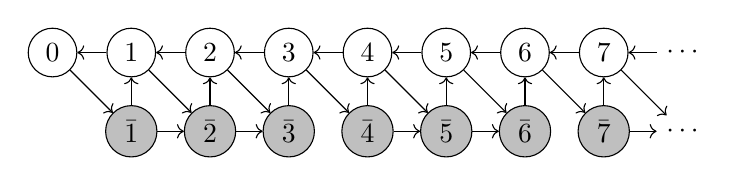
\begin{tikzpicture}
		% nodes
		\batchfirstnodes
		
		% edges
		\foreach \i/\j in {0/1, 1/2, 2/3, 3/4, 4/5, 5/6, 6/7, 7/8} {
			\draw[->] (\j) -- (\i);
			\draw[->] (\i) -- (bar\j);
		}
		
		\foreach \i/\j in {1/2, 2/3, 4/5, 5/6, 7/8} {
			\draw[->] (bar\i) -- (bar\j);
		}
		
		\foreach \i/\j in {0/1, 1/2, 2/3, 3/4, 4/5, 5/6, 6/7} {
			\draw[->] (bar\j) -- (\j);
		}
		\end{tikzpicture}
		\caption{Transition diagram graph~$G$.}
		\label{fig:batch1-diagram}
	\end{subfigure} \\[.4cm]
	\begin{subfigure}{\textwidth}
		\centering
		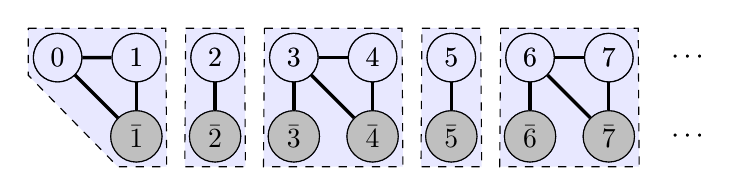
\begin{tikzpicture}
		% nodes
		\batchfirstnodes
		
		% edges
		\foreach \i in {1, 2, ..., 7} {
			\draw (\i) -- (bar\i);
		}
		
		\foreach \i/\j in {3/bar4, 6/bar7} {
			\draw (\i) -- (\j);
		}
		
		\draw (1) -- (0) -- (bar1);
		\draw (3) -- (4) (6) -- (7);
		
		% cliques
		\batchfirstcliques
		
		% nodes
		\batchfirstnodes
		
		% first-level cuts
		\foreach \i in {1, 2, ..., 7} \draw[newedge] (\i) -- (bar\i);
		\foreach \i/\j in {3/bar4, 6/bar7} \draw[newedge] (\i) -- (\j);
		\draw[newedge] (1) -- (0) -- (bar1);
		\draw[newedge] (3) -- (4) (6) -- (7);
		\end{tikzpicture}
		\caption{First-level cut graph $C_1(G)$. Edges (solid lines) connect nodes that are in an S-product-form relationship. Dashed contours outline connected components of~$C_1(G)$.}
		\label{fig:batch1-cut1}
	\end{subfigure} \\[.4cm]
	\begin{subfigure}{\textwidth}
		\centering
		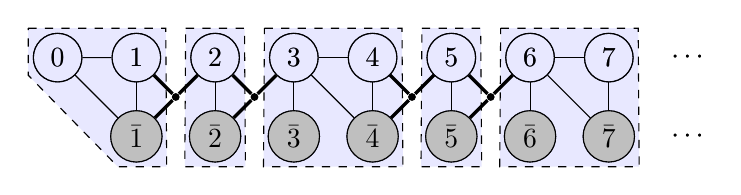
\begin{tikzpicture}
		% nodes
		\batchfirstnodes
		
		% cliques
		\batchfirstcliques
		
		% first-level cuts
		\foreach \i in {1, 2, ..., 7} \draw (\i) -- (bar\i);
		\foreach \i/\j in {3/bar4, 6/bar7} \draw (\i) -- (\j);
		\draw (1) -- (0) -- (bar1);
		\draw (3) -- (4) (6) -- (7);
		
		% second-level cuts
		\foreach \i\j in {1/2, 2/3, 4/5, 5/6} {
			\node[circle, fill, inner sep=1pt]
			(dot) at ($(\i)!.5!(bar\j)$) {};
			\draw[newedge] (dot) -- (\i) (dot) -- (bar\i) (dot) -- (\j);
		}
		
		% nodes
		\batchfirstnodes
		\end{tikzpicture}
		\caption{Second-level cut graph~$C_2(G)$. Solid lines intersecting at a dot represent second-level cuts, showing the source nodes of the cut.}
		\label{fig:batch1-cut2}
	\end{subfigure}
	\caption{Queue with batch arrivals, first version.}
	\label{fig:batch1}
\end{figure}

\begin{table}[ht]
	\centering
	\begin{tabular}{c|l|l}
		Level & Nodes & Equation \\
		\hline
		\multirow{11}{.2cm}{1}
		& $0$ and $1$
		& $\pi(0) q_{0, \bar 1} = \pi(1) q_{1, 0}$ \\
		& $0$ and $\bar 1$
		& $\pi(0) q_{0, \bar 1} = \pi(\bar 1) (q_{\bar 1, 1} + q_{\bar 1, \bar 2})$ \\
		& $1$ and $\bar 1$
		& $\pi(1) q_{1, 0} = \pi(\bar 1) (q_{\bar 1, 1} + q_{\bar 1, \bar 2})$ \\
		& $2$ and $\bar 2$
		& $\pi(2) q_{2, 1} = \pi(\bar 2) (q_{\bar 2, 2} + q_{\bar 2, \bar 3})$ \\
		& $3$ and $\bar 3$
		& $\pi(3) q_{3, 2} = \pi(\bar 3) (q_{\bar 3, 3} + q_{\bar 3, \bar 2})$ \\
		& $3$ and $4$
		& $\pi(3) q_{3, \bar 4} = \pi(4) q_{4, 3}$ \\
		& $4$ and $\bar 4$
		& $\pi(4) q_{4, 3} = \pi(\bar 4) (q_{\bar 4, 4} + q_{\bar 4, \bar 3})$ \\
		& $5$ and $\bar 5$
		& $\pi(5) q_{5, 4} = \pi(\bar 5) (q_{\bar 5, 5} + q_{\bar 5, \bar 4})$ \\
		& $6$ and $\bar 6$
		& $\pi(6) q_{6, 5} = \pi(\bar 6) (q_{\bar 6, 6} + q_{\bar 6, \bar 5})$ \\
		& $6$ and $7$
		& $\pi(6) q_{6, \bar 7} = \pi(7) q_{7, 6}$ \\
		& $7$ and $\bar 7$
		& $\pi(7) q_{7, 6} = \pi(\bar 7) (q_{\bar 7, 7} + q_{\bar 7, \bar 6})$ \\
		\hline
		\multirow{4}{.2cm}{2}
		& $\{1, \bar 1\}$ and $2$
		& $\pi(1) q_{1, \bar 2} + \pi(\bar 1) q_{\bar 1, \bar 2} = \pi(2) q_{2, 1}$ \\
		& $\{2, \bar 2\}$ and $3$
		& $\pi(2) q_{2, \bar 3} + \pi(\bar 2) q_{\bar 2, \bar 3} = \pi(3) q_{3, 2}$ \\
		& $\{4, \bar 4\}$ and $5$
		& $\pi(4) q_{4, \bar 5} + \pi(\bar 4) q_{\bar 4, \bar 5} = \pi(5) q_{5, 4}$ \\
		& $\{5, \bar 5\}$ and $6$
		& $\pi(5) q_{5, \bar 6} + \pi(\bar 5) q_{\bar 5, \bar 6} = \pi(6) q_{6, 5}$
	\end{tabular}
	\caption{Cuts associated with
		the single-server queue batch example of \Cref{fig:batch1}.}
	\label{tab:batch1}
\end{table}

We consider the embedded DTMC of the system, examining moments when jobs enter the system or complete. 
\Cref{fig:batch1-diagram} shows the graph~$G$ underlying the Markov chain for this batch-arrivals system. It is infinite in one direction,
in contrast to the finite graph we considered in \Cref{sec:msj-example}.
In the same spirit as \Cref{sec:msj-example},
there are two kinds of states: during a batch, when a job has just arrived, and in the bulk of time, when jobs may complete or a new batch may arrive. We denote states by the number of jobs in the system, and by whether the state is immediately-post-arrival, shown in grey, or spanning a nonzero amount of time, shown in white.
An overbar denotes an immediately-post-arrival state.
For instance, state $4$ has four jobs in the system, and jobs may complete or a new batch may begin.
State $\bar{7}$ has seven jobs, and a batch of arrivals is ongoing.
When a batch ends, the system transitions from the immediately-post-arrival state to the corresponding general-time state, such as from state $\bar{2}$ to state $2$.

\Cref{fig:batch1-cut1} shows the first-level cut graph $C_1(G)$ corresponding to this graph. For instance, there is a first-level cut between nodes $3$ and $\bar{4}$.
This cut partitions the graph into two subsets: $A_{\bar{4}}(G {\setminus} 3) = \{\bar{4}\}$, and $A_3(G {\setminus} \bar{4}) = V \setminus \{\bar{4}\}$.
This cut gives rise to an S-product form relationship between nodes $3$ and $\bar{4}$. More first-level cuts and corresponding S-product-form relationships are listed in \Cref{tab:batch1}.

The connected components of $C_1(G)$, illustrated with dashed outlines in \Cref{fig:batch1-cut1}, each contain two to four vertices. Between these components, there exist second-level cuts, as shown in \Cref{fig:batch1-cut2}.
For instance, between components $K_1 = \{2, \bar{2}\}$ and $K_2 = \{3, \bar{3}, 4, \bar{4}\}$,
there exists a cut with sources $I = K_1 = \{2, \bar{2}\}$ and $J = \{3\}, J \subseteq K_2$. Correspondingly, $K_1$ and $K_2$ are joint-ancestor free.

This cut partitions the graph into two subsets: $A_I(G {\setminus} J) = \{0, 1, \bar{1}, 2, \bar{2}\},$
and $A_J(G {\setminus} I) = \{3, \bar{3}, 4, \bar{4}, 5, \bar{5}, \ldots\}$.
Due to this second-level cut, the graph induces an SPS-product-form relationship between each pair of vertices in $K_1$ and $K_2$, by \Cref{lem:second-level-sps}. Each connected component has a second-level cut with each of its neighbors, as shown in \Cref{fig:batch1-cut2} and in \Cref{tab:batch1}, so the Markov chain has a PSPS-product-form.

The same is true if one varies the parameters defining the system and its Markov chain, for instance by changing the multiplier 3 that truncates the batches to some other multiplier, or truncating the batches at an arbitrary sequence of cutoff values.



\subsection{Queue with batch arrivals: unstructured}

Finally, we give an example of a queueing system with a positive number of first-level cuts, second-level, third-level, and so forth, but for which the entire graph is not connected via any finite level of cuts.

Consider a single-server queueing system with unstructured batch arrivals, of size either 1 or 2. Jobs arrive in batches of size 1 with probability $p_1$ and 2 with probability $p_2$, with $p_1 + p_2 = 1$. Jobs are indistinguishable, with exponential service time. Batch arrivals occur according to a Poisson process.

We examine the embedded DTMC of the system, examining moments when jobs enter the system or complete. We use the same state representation as in \Cref{sec:batch1}.
\Cref{fig:batch2-diagram} shows the graph~$G$ underlying the Markov chain for this batch-arrivals system. \Cref{fig:batch2-cut1} shows the first-level cut graph $C_1(G)$ corresponding to this graph. \Cref{tab:batch2-1} lists some such cuts and the corresponding S-product form relationships.

\newcommand{\batchsecond}{
	\foreach \i in {0, 1, ..., 5} {
		\node[state] (\i) at (\i, 0) {$\i$};
	}
	
	\foreach \i in {1, 3, 5} {
		\node[phantom] (bar\i) at (\i, 1) {$\bar \i$};
	}
	
	\foreach \i in {2, 4} {
		\node[phantom] (bar\i) at (\i, -1) {$\bar \i$};
	}
	
	\node (6) at (6, 0) {$\cdots$};
	\node (bar6) at (6, -1) {$\cdots$};
}

\begin{figure}[htb]
	\begin{subfigure}{.49\textwidth}
		\centering
		\begin{tikzpicture}
		% nodes
		\batchsecond
		
		% edges
		\foreach \i/\j/\k in {0/1/2, 1/2/3, 2/3/4, 3/4/5, 4/5/6} {
			\draw[->] (\j) -- (\i);
			\draw[->] (\i) -- (bar\j);
			\draw[->] (bar\j) -- (\j);
			\draw[->] (bar\j) -- (\k);
		}
		\draw[->] (6) -- (5);
		\draw[->] (bar6) -- (5);
		\end{tikzpicture}
		\caption{Transition diagram~$G$.}
		\label{fig:batch2-diagram}
	\end{subfigure} \hfill
	\begin{subfigure}{.49\textwidth}
		\centering
		\begin{tikzpicture}
		% nodes
		\batchsecond
		
		% first-level cuts
		\draw[newedge] (1) -- (0) -- (bar1) -- (1) -- (bar2);
		\draw[newedge] (2) -- (bar3);
		\draw[newedge] (3) -- (bar4);
		\draw[newedge] (4) -- (bar5);
		\draw[newedge] (5) -- (bar6);
		\end{tikzpicture}
		\caption{First-level cut graph~$C_1(G)$.}
		\label{fig:batch2-cut1}
	\end{subfigure} \\[.4cm]
	\begin{subfigure}{.49\textwidth}
		\centering
		\begin{tikzpicture}
		% nodes
		\batchsecond
		
		% first-level cuts
		\draw (1) -- (0) -- (bar1) -- (1) -- (bar2);
		\draw (2) -- (bar3);
		\draw (3) -- (bar4);
		\draw (4) -- (bar5);
		\draw (5) -- (bar6);
		
		% second-level cuts
		\node[circle, fill, inner sep=1pt] (dot) at ($(1)!.5!(2)$) {};
		\draw[newedge] (dot) -- (bar1) (dot) -- (2) (dot) -- (bar2);
		\end{tikzpicture}
		\caption{Second-level cut graph $C_2(G)$.}
		\label{fig:batch2-cut2}
	\end{subfigure}
	\begin{subfigure}{.49\textwidth}
		\centering
		\begin{tikzpicture}
		% nodes
		\batchsecond
		
		% first-level cuts
		\draw (1) -- (0) -- (bar1) -- (1) -- (bar2);
		\draw (2) -- (bar3);
		\draw (3) -- (bar4);
		\draw (4) -- (bar5);
		\draw (5) -- (bar6);
		
		% second-level cuts
		\node[circle, fill, inner sep=1pt] (dot) at ($(1)!.5!(2)$) {};
		\draw (dot) -- (bar1) (dot) -- (2) (dot) -- (bar2);
		
		% third-level cuts
		\node[circle, fill, inner sep=1pt] (dot) at ($(2)!.5!(3)$) {};
		\draw[newedge] (dot) -- (bar2) (dot) -- (3) (dot) -- (bar3);
		\end{tikzpicture}
		\caption{Third-level cut graph $C_3(G)$.}
		\label{fig:batch2-cut3}
	\end{subfigure}
	\caption{Queue with batch arrivals, second version.}
	\label{fig:batch2}
\end{figure}

In contrast to the structured batch setting in \Cref{sec:batch1}, there are very few second-level cuts in this graph. In fact, the only second level cuts are between subsets of the two leftmost components of the cut graph, namely $K_1 = \{0, 1, \bar{1}, \bar{2}\}$ and $K_2 = \{2, \bar{3}\}$, as shown in \Cref{fig:batch2-cut2}. 
A narrow second-level cut exists between these components, namely $A_{K_1}(G {\setminus} K_2) = K_1$ and $A_{K_2}(G {\setminus} K_1) = G {\setminus} K_1$. This cut has source $(\{\bar{1}, \bar{2}\}, \{2\})$, as shown in \Cref{fig:batch2-cut2}.

\begin{table}[ht]
	\centering
	\begin{tabular}{c|l|l}
		Level & Nodes & Equation \\
		\hline
		\multirow{6}{.2cm}{1}
		& $0$ and $1$
		& $\pi(0) q_{0, \bar 1} = \pi(1) q_{1, 0}$ \\
		& $0$ and $\bar 1$
		& $\pi(0) q_{0, \bar 1} = \pi(\bar 1) (q_{\bar 1, 1} + q_{\bar 1, 2})$ \\
		& $1$ and $\bar 1$
		& $\pi(1) q_{1, 0} = \pi(\bar 1) (q_{\bar 1, 1} + q_{\bar 1, 2})$ \\
		& $2$ and $\bar 3$
		& $\pi(2) q_{2, \bar 3} = \pi(\bar3) (q_{\bar 3, 3} + q_{\bar 3, 4})$ \\
		& $3$ and $\bar 4$
		& $\pi(3) q_{3, \bar 4} = \pi(\bar4) (q_{\bar 4, 4} + q_{\bar 4, 5})$ \\
		& $4$ and $\bar 5$
		& $\pi(4) q_{4, \bar 5} = \pi(\bar5) (q_{\bar 5, 5} + q_{\bar 5, 6})$ \\
		\hline
		2 & $\{\bar 1, \bar 2\}$ and $2$
		& $\pi(\bar 1) q_{\bar 1, 2} 
		+ \pi(\bar 2) (q_{\bar 2, 2} + q_{\bar 2, 3}) = \pi(2) q_{2, 1}$ \\
		\hline
		3 & $\{\bar 2, \bar 3\}$ and $3$
		& $\pi(\bar 2) q_{\bar 2, 3} +
		\pi(\bar 3) (q_{\bar 3, 3} + q_{\bar 3, 4}) = \pi(3) q_{3, 2}$
	\end{tabular}
	\caption{Cuts associated with
		the single-queue batch example of \Cref{fig:batch2}.}
	\label{tab:batch2-1}
\end{table}

This cut implies an SPS product-form relationship between every pair of vertices $i \in K_1$ and $j \in K_2$. The key equation for defining that SPS relationship is the second-level equation in \Cref{tab:batch2-1}.

Note that other subsets of $K_1$ and $K_2$ also form broad second-level cuts, such as $\{\bar{1}, 1\} \subset K_1, \{2\} \subset K_2$. This is the behavior predicted by \Cref{conj:second-level}, which states that broad second level cuts will only exist between subsets of connected components that also have narrow second-level cuts, but that the sources may differ.

We can recursively define third-level cuts based on the connected components of the second-level cut graph. However, as the second-level cut graph only adds a single hyperedge, the only difference between the first-level components and the second-level components is that $K_1$ and $K_2$ are combined into a single component. As result, there is only a single third-level cut, shown in \Cref{fig:batch2-cut3}. We can continue on to higher and higher levels of the cut graph, adding a single cut each time.

Corresponding to the fact that the $n$th cut graph is not fully connected for any finite level $n$, the Markov chain does not exhibit (PS)$^n$ or S(PS)$^n$ product form for any finite level $n$. However, any two specific nodes $i, j \in V$ are connected in some (potentially large) level of the cut graph, and are in an S(PS)$^n$ product-form relationship for some correspondingly large $n$.





\paragraph*{Acknowledgements}

Thank you to Jean-Michel Fourneau for pointing out \cite{F87} in an informal discussion on queueing systems with product-form stationary distributions.





\appendix
	
	



\section{Cliques in the cut graph} \label{app:clique}

As announced in \Cref{sec:cut-graph},
\Cref{theo:clique} below gives a necessary and sufficient condition
for the existence of a clique in the cut graph
of a formal Markov chain.
This condition can be seen as an extension of \Cref{prop:jaf-cuts-1},
which corresponds to a clique of size~2.

\begin{theorem} \label{theo:clique}
	Consider a formal Markov chain $G = (V, E)$
	and a set $K \subseteq V$ of $n \ge 2$ nodes.
	Also let $V_i = A_i(G {\setminus} (K {\setminus} \{i\}))$ for each $i \in K$,
	and consider the directed graph $Q = (K, L)$ where
	$L = \{(i, j) \in K \times K: i \neq j~\text{and}~E \cap (V_i \times V_j) \neq \emptyset\}$.
	Then:
	\begin{enumerate}[(i)]
		\item \label{item:clique-1} $V = \bigcup_{i \in K} V_i$.
		\item \label{item:clique-2} The following statements are equivalent:
		\begin{enumerate}
			\item \label{item:clique-21}
			$K$ is a clique in $C_1(G)$.
			\item \label{item:clique-22}
			$(V_i)_{i \in K}$ is a partition of~$V$
			and $Q$ is a directed cycle.
		\end{enumerate}
		\item \label{item:clique-3}
		If the equivalent statements of \eqref{item:clique-2} are satisfied
		then, for each $i, j \in K$,
		the $i, j$-sourced cut is $(S, T)$ with
		$S = \bigcup_{k \in A_i(Q {\setminus} j)} V_k$
		and $T = \bigcup_{k \in A_j(Q {\setminus} i)} V_k$.
	\end{enumerate}
\end{theorem}

\Cref{theo:clique} is illustrated in \Cref{fig:clique}
with a $9$-node formal Markov chain
whose cut graph contains the clique $K = \{1, 5, 6, 8, 9\}$.
Indeed, condition~\eqref{item:clique-22} of \Cref{theo:clique} is satisfied:
the sets $V_1$, $V_5$, $V_6$, $V_8$, and $V_9$ are disjoint,
and the quotient graph~$Q$
as defined in \Cref{theo:clique} is a cycle
visiting $V_1$, $V_5$, $V_6$, $V_8$, and $V_9$, in this order%
\footnote{
	Note that we identify each subset $V_i$ with its representative vertex $i \in K$. While formally $Q$ is defined with $K$ as its set of vertices,
	we equivalently think of it as having the family $(V_i)_{i \in K}$ as vertices.
}.
Intuitively, the nodes in~$K$ act as \emph{no-return points} in the graph~$G$
in the sense that, once the set $V_i$ has been exited (necessarily via~$i$) for some $i \in K$,
the only way of returning to this set is by traversing the graph~$G$
consistently with the cycle~$Q$.
Saying that the sets $V_1$, $V_5$, $V_6$, $V_8$, and $V_9$ are pairwise disjoint
(and therefore form a partition of~$V$)
is equivalent to saying that node~$i$ is the only exit point from set $V_i$, for each $i \in K$.
Focusing for instance on nodes~$5$ and $8$,
the $5, 8$-sourced cut is given by $(V_5 \cup V_1 \cup V_9, V_8 \cup V_6)$.

\begin{figure}[t]
	\centering
	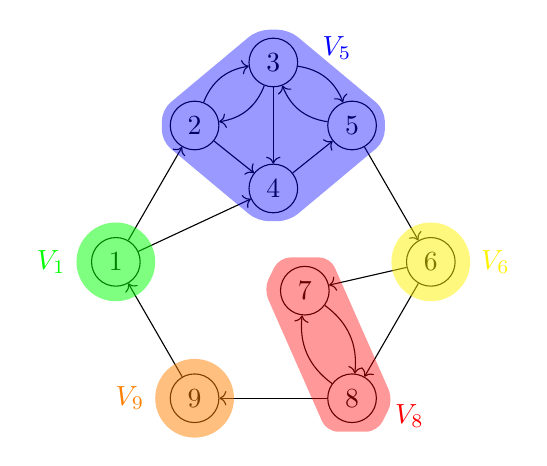
\begin{tikzpicture}
	% place nodes
	\foreach \a in {1, 2, ..., 6} {
		\node[state] (\a) at (180-\a*360/6: 2cm) {\phantom{\a}};
	}
	\node[state] (7) at ($(1)!.5!(2)+(0, .8cm)$) {\phantom{7}};
	\node[state] (8) at ($(1)!.5!(2)+(0, -.8cm)$) {\phantom{8}};
	\node[state] (9) at ($(3)!.5!(4)+(-1.1cm, .5cm)$) {\phantom{9}};
	
	% draw edges
	\draw (6) edge[->] (1);
	\draw (6) edge[->] (8);
	\draw (1) edge[->, bend left] (7);
	\draw (1) edge[->] (8);
	\draw (7) edge[->, bend left] (1);
	\draw (7) edge[->] (8);
	\draw (7) edge[->, bend left] (2);
	\draw (8) edge[->] (2);
	\draw (2) edge[->, bend left] (7);
	\draw (2) edge[->] (3);
	\draw (3) edge[->] (4);
	\draw (3) edge[->] (9);
	\draw (9) edge[->, bend left] (4);
	\draw (4) edge[->, bend left] (9);
	\draw (4) edge[->] (5);
	\draw (5) edge[->] (6);
	
	% renumber nodes and draw them
	\node at (6) {1};
	\node at (1) {2};
	\node at (7) {3};
	\node at (8) {4};
	\node at (2) {5};
	\node at (3) {6};
	\node at (9) {7};
	\node at (4) {8};
	\node at (5) {9};
	
	% draw the ancestor sets
	\fill[blue, opacity=.4, rounded corners]
	($(1.west)+(-.1cm, 0)$) -- ($(1.west)+(-.1cm, .2cm)$)
	-- ($(7.north)+(-.2cm, .1cm)$) -- ($(7.north)+(.2cm, .1cm)$)
	-- node[midway, right, above, opacity=1] {$V_5$} ($(2.east)+(.1cm, .2cm)$) -- ($(2.east)+(.1cm, -.2cm)$)
	-- ($(8.south)+(.2cm, -.1cm)$) -- ($(8.south)+(-.2cm, -.1cm)$)
	-- ($(1.west)+(-.1cm, -.2cm)$) -- ($(1.west)+(-.1cm, 0)$);
	
	\fill[yellow, semitransparent] (3) circle[radius=.5cm];
	\node[yellow, right] at ($(3.east)+(.2cm, 0)$) {$V_6$};
	
	\fill[red,  opacity=.4, rounded corners]
	($(4.south east)+(0, -.2cm)$) -- ($(4.south east)+(.1cm, -.2cm)$)
	-- node[midway, right, opacity=1] {$V_8$} ($(4.south east)+(.3cm, .2cm)$)
	-- ($(9.north east)+(.1cm, .2cm)$) -- ($(9.north west)+(-.1cm, .2cm)$) -- ($(9.north west)+(-.3cm, -.2cm)$)
	-- ($(4.south west)+(-.1cm, -.2cm)$) -- ($(4.south west)+(0, -.2cm)$);
	
	\fill[orange, semitransparent] (5) circle[radius=.5cm];
	\node[orange, left] at ($(5.west)+(-.2cm, 0)$) {$V_9$};
	
	\fill[green, semitransparent] (6) circle[radius=.5cm];
	\node[green, left] at ($(6.west)+(-.2cm, 0)$) {$V_1$};
	\end{tikzpicture}
	\caption{A formal Markov chain whose cut graph contains the clique $\{1, 5, 6, 8, 9\}$.}
	\label{fig:clique}
\end{figure}

\begin{proof}[Proof of \Cref{theo:clique}]
	We prove each statement one after another.
	
	\medskip
	
	\noindent \eqref{item:clique-1}
	Let $k \in V$.
	Since $G$ is strongly connected,
	there exists a directed path $k_1, k_2, \ldots, k_n$,
	with $k_1 = k$ and $k_n \in K$.
	Then $k \in V_{k_p}$ with $p = \min\{q \in \{1, 2, \ldots, n\} | k_q \in K\}$.
	
	\medskip
	
	\noindent \eqref{item:clique-2}
	We prove each direction of the equivalence separately.
	
	\noindent
	First assume that \eqref{item:clique-21} is satisfied:
	$K$ is a clique in $C_1(G)$.
	By \Cref{prop:jaf-cuts-1},
	it means that $A_i(G {\setminus} j) \cap A_j(G {\setminus} i) = \emptyset$ for each $i, j \in K$.
	We now verify the two parts of \eqref{item:clique-22}:
	\begin{itemize}
		\item $(V_i)_{i \in K}$ is a partition of~$V$:
		For each $i, j \in K$, we have $V_i \cap V_j = \emptyset$ because
		$V_i \subseteq A_i(G {\setminus} j)$,
		$V_j \subseteq A_j(G {\setminus} i)$,
		and $A_i(G {\setminus} j) \cap A_j(G {\setminus} i) = \emptyset$.
		Therefore, $(V_i)_{i \in K}$ is a family of pairwise disjoint sets.
		Combining this with~\eqref{item:clique-1}
		implies that $(V_i)_{i \in K}$ is a partition of~$V$.
		\item $Q$ is a directed cycle:
		$Q$ is strongly connected
		because $G$ is and $(V_i)_{i \in V}$ covers~$V$.
		It remains to be proved that, for each $i \in K$,
		there is at most one~$j \in K {\setminus} \{i\}$
		such that $(i, j) \in L$.
		First observe that, for each $i, j \in K$,
		we have $E \cap (V_i \times V_j) \subseteq \{i\} \times V_j$
		because $V_i \subseteq A_i(G {\setminus} j)$,
		$V_j \subseteq A_j(G {\setminus} i)$, and
		\eqref{item:clique-21} implies that
		$(A_i(G {\setminus} j), A_j(G {\setminus} i))$
		is an $i, j$-sourced cut.
		Now assume for the sake of contradiction that
		there are $j, j' \in K$, with $j \neq j'$,
		such that $(i, j) \in L$ and $(i, j') \in L$.
		Combined with the previous observation,
		it follows there exist $k \in V_j$ and $k' \in V_{j'}$
		such that $(i, k) \in E$ and $(i, k') \in E$.
		Recalling the definitions of $V_j$ and $V_{j'}$,
		we conclude that $i \in A_j(G {\setminus} j') \cap A_{j'}(G {\setminus} j)$,
		By \Cref{prop:jaf-cuts-1},
		this contradicts our assumption that there is a $j, j'$-sourced cut.
	\end{itemize}
	
	\noindent
	Now assume that \eqref{item:clique-22} is satisfied, i.e.,
	$(V_i)_{i, \in K}$ is a partition of~$V$
	and $Q$ is a directed cycle.
	We proceed step-by-step.
	\begin{enumerate}[(A)]
		\item \label{intermediary-1}
		We first verify that,
		for each $(i, j) \in L$, we have
		$E \cap (V_i \times V_j) \subseteq \{i\} \times V_j$,
		i.e., edges in~$G$ from~$V_i$ to~$V_j$ necessarily have source node~$i$.
		Let $(i, j) \in L$.
		Assume for the sake of contradiction that
		there exist $k \in V_i {\setminus} \{i\}$
		and $\ell \in V_j$
		such that $(k, \ell) \in E$.
		Then there exists a path from~$k$ to~$j$
		(through $\ell$) that does not visit
		any node in~$K {\setminus} \{j\}$,
		meaning that $k \in V_j$,
		which is impossible since
		$k \in V_i$ and $V_i \cap V_j = \emptyset$.
	\end{enumerate}
	Now let $i, j \in K$,
	$S = \bigcup_{k \in A_i(Q {\setminus} j)} V_k$,
	and $T = \bigcup_{k \in A_j(Q {\setminus} i)} V_k$.
	Our end goal is to prove that $(S, T)$
	is an $i, j$-sourced cut.
	\begin{enumerate}[(A)]
		\setcounter{enumi}{1}
		\item \label{intermediary-3}
		We know that $(S, T)$ is a partition of~$V$ because
		$(A_i(Q {\setminus} j), A_j(Q {\setminus} i))$
		is a partition of~$K$
		(since~$Q$ is a directed cycle)
		and $(V_k)_{k \in k}$ is a partition of~$V$.
		\item \label{intermediary-2}
		Let us prove that,
		for each $k \in A_i(Q {\setminus} j)$,
		every path in~$G$
		from any node in~$V_k$ to node~$j$ visits node~$i$.
		Let $k \in A_i(Q {\setminus} j)$ and $\ell \in V_k$.
		Consider any path $\ell_1, \ell_2, \ldots, \ell_n$ in~$G$
		such that $\ell_1 = \ell$ and $\ell_n = j$.
		For each $p \in \{1, 2, \ldots, n\}$,
		let $k_p$ denote the unique node in~$K$
		such that $\ell_p \in V_{k_p}$;
		we have in particular $k_1 = k$ and $k_n = j$.
		By definition of~$Q$, for each $p \in \{1, 2, \ldots, n-1\}$,
		we have either $k_p = k_{p+1}$ or $(k_p, k_{p+1}) \in L$,
		i.e., the sequence of distinct nodes
		in $k_1, k_2, \ldots, k_n$ forms a path in~$Q$.
		Since $Q$ is a directed cycle
		and $k \in A_i(Q {\setminus} j)$,
		the only path in~$Q$ from~$k_1 = k$ to~$k_n = j$ visits~$i$.
		Hence, there is~$q \in \{1, 2, \ldots, n-1\}$
		such that $k_q = i$,
		and we can define
		$p = \max\{q \in \{1, 2, \ldots, n\}: k_q = i\}$.
		We know that $p \le n-1$ since $k_n = j \neq i$.
		We obtain $(k_p, k_{p+1}) \in L$,
		so that by~\ref{intermediary-1}
		we have necessarily $\ell_p = i$.
		\item \label{intermediary-4}
		Let us now prove that
		$A_j(G {\setminus} i) \subseteq T$,
		i.e., if $\ell \in S = V {\setminus} T$
		then $\ell \notin A_j(G {\setminus} i)$.
		Let $\ell \in S$.
		By definition of~$S$,
		there is $k \in A_i(Q {\setminus} j)$
		so that $\ell \in V_k$.
		By~\ref{intermediary-2}, every path in~$G$
		from node~$\ell$ to node~$j$ visits node~$i$
		(and such a path exists since $G$ is strongly connected).
		By definition of $A_j(G {\setminus} i)$,
		this means that $\ell \notin A_j(G {\setminus} i)$.
		\item Putting all the pieces together,
		we have that $A_j(G {\setminus} i) \subseteq T$ (by \ref{intermediary-4}),
		$A_i(G {\setminus} j) \subseteq S$ (by symmetry),
		$(S, T)$ is a partition of~$V$ (by \ref{intermediary-3}),
		and $A_i(G {\setminus} j) \cup A_j(G {\setminus} i) = V$
		(by \Cref{lem:jaf-cuts}\eqref{prop:ancestors-1}).
		It follows that $A_i(G {\setminus} j) = S$ and $A_j(G {\setminus} i) = T$,
		and that $A_i(G {\setminus} j) \cap A_j(G {\setminus} i) = \emptyset$,
		i.e., nodes~$i$ and~$j$ are joint-ancestor free.
		By \Cref{prop:jaf-cuts-1},
		we conclude that
		$(A_i(G {\setminus} j), A_j(G {\setminus} i)) = (S, T)$
		is the $i, j$-sourced cut.
	\end{enumerate}
	
	\medskip
	
	\noindent \eqref{item:clique-3}
	This is a by-product of the proof of \eqref{item:clique-2}.
\end{proof}

\section{Second-level cuts: Progress towards \Cref{conj:second-level}}
\label{app:second-level}

In \Cref{sec:paths-cut-graph}, we prove intermediary results
that are then applied in \Cref{sec:expanding-case}
to prove \Cref{theo:induction-step-1}.

\subsection{Paths in the cut graph}
\label{sec:paths-cut-graph}

Let us first study the behavior of paths $i_1, i_2, \ldots, i_n$ in the cut graph $C_1(G)$,
where each pair of neighboring vertices in the path is joint-ancestor free.
We are interested in the joint-ancestor freeness of the two terminal nodes in the path,
$i_1$ and $i_n$.
We show that the endpoints $i_1$ and $i_n$ cannot share a joint ancestor in the subgraph graph $G {\setminus} \{i_2, i_3, \ldots i_{n-1}\}$.

First, for the purpose of induction, we prove this claim for length-3 paths:

\begin{lemma} \label{lem:path-3}
	Consider a directed graph $G = (V, E)$
	and three nodes $i_1, i_2, i_3 \in V$
	such that $i_1$ and $i_2$ are joint-ancestor free
	(i.e., $A_{i_1}(G {\setminus} i_2)
	\cap A_{i_2}(G {\setminus} i_1) = \emptyset$)
	and $i_2$ and $i_3$ are joint-ancestor free
	(i.e., $A_{i_2}(G {\setminus} i_3)
	\cap A_{i_3}(G {\setminus} i_2) = \emptyset$).
	Then $A_{i_1}(G {\setminus} \{i_2, i_3\})
	\cap A_{i_3}(G {\setminus} \{i_1, i_2\}) = \emptyset$.
\end{lemma}

\begin{proof}
	Assume for the sake of contradiction that
	$A_{i_1}(G {\setminus} \{i_2, i_3\})
	\cap A_{i_3}(G {\setminus} \{i_1, i_2\}) \neq \emptyset$,
	and let $k \in A_{i_1}(G {\setminus} \{i_2, i_3\})
	\cap A_{i_3}(G {\setminus} \{i_1, i_2\})$.
	We will prove that either
	$k \in A_{i_2}(G {\setminus} i_1)$
	or $k \in A_{i_2}(G {\setminus} i_3)$,
	which will contradict our assumption that
	$i_1$ and $i_2$ are joint-ancestor free
	and $i_1$ and $i_3$ are joint-ancestor free.
	Since $G$ is strongly connected,
	there is a path $p = p(k \to i_2)$.
	We now make a case disjunction.
	
	First, suppose that $p(k \to i_2)$ either does not visite node~$i_1$ or does not visit node~$i_3$.
	If $p(k \to i_2)$ does not visit node $i_1$, then $k \in A_{i_2}(G {\setminus} i_1)$.
	Since $k \in A_{i_1}(G \setminus \{i_2, i_3\}) \subseteq A_{i_1}(G \setminus i_2)$, this contradicts our assumption that nodes $i_1$ and $i_2$ are joint-ancestor free.
	If $p(k \to i_2)$ does not visit node $i_3$, then $k \in A_{i_2}(G {\setminus} i_3)$, which leads to a similar contradiction regarding nodes~$i_2$ and~$i_3$.
	
	On the other hand, suppose that $p(k \to i_2)$ visits both $i_1$ and $i_3$.
	Let us consider~$p'$, the last portion of~$p$ beginning at the last visit to either $i_1$ or $i_3$.
	Without loss of generality, suppose $p'$ begins at $i_1$
	and reaches $i_2$ without visiting $i_3$.
	Since we assumed that $k \in A_{i_1}(G {\setminus} \{i_2, i_3\})$,
	concatenating $p(k \to i_1 {\setminus} \{i_2, i_3\})$ and $p'$
	gives us a path from $k$ to $i_2$ without visiting $i_3$.
	So $k \in A_{i_2}(G {\setminus} i_3)$,
	which as explained before leads to a contradiction.
	
	In every case, we have a contradiction to either our assumption that $i_1$ and $i_2$ are joint-ancestor free, or that $i_2$ and $i_3$ are joint-ancestor free.
	%    
	Thus, our initial assumption much be wrong: There is no node $k$ in $A_{i_1}(G {\setminus} \{i_2, i_3\})
	\cap A_{i_3}(G {\setminus} \{i_1, i_2\})$, as desired. \qedhere
\end{proof}

Next, we build inductively on this result to handle paths of arbitrary lengths.

\begin{lemma} \label{lem:path-n}
	Consider a directed graph $G = (V, E)$
	and a sequence of $n \ge 3$ distinct nodes
	$i_1, i_2, \ldots, i_n$
	such that $i_p$ and $i_{p+1}$
	are joint-ancestor free
	for each $p \in \{1, 2, \ldots, n-1\}$.
	Then $A_{i_1}(G {\setminus} \{i_2, i_3, \ldots, i_n\})
	\cap A_{i_n}(G {\setminus} \{i_1, i_2, \ldots, i_{n-1}\})
	= \emptyset$.
\end{lemma}

\begin{proof}
	We make a proof by induction over~$n$,
	using \Cref{lem:path-3} as a base case for $n = 3$.
	
	Let $n \ge 4$ and assume the induction assumption is true for each $p \in \{3, 4, \ldots, n-1\}$.
	Assume for the sake of contradiction that
	the conclusion does not hold,
	i.e., there exist $k \in V$ and two paths
	$p_{(a)} = p(k \to i_1 {\setminus} \{i_2, i_3, \ldots, i_n\})$
	and $p_{(b)} = p(k \to i_n {\setminus} \{i_1, i_2, \dots, i_{n-1}\})$.
	
	Since $G$ is strongly connected,
	we know that at least one of the following is true:
	there is a path $p_{(1)} = p(i_1 \to i_{n-1} {\setminus} i_n)$,
	or there is a path $p_{(2)} = p(i_n \to i_{n-1} {\setminus} i_1)$.
	To see why, consider a path $x$ from $i_1$ to $i_{n-1}$. If the path $x$ avoids $i_n$, $x$ is $p_{(1)}$, and we have the first case. If the path visits $i_n$, the tail of the path $x$ starting at its visit to $i_n$ is $p_{(2)}$, satisfying the second case.
	
	Let us consider each case in turn:
	\begin{itemize}
		\item Suppose there is a path $p_{(1)} = p(i_1 \to i_{n-1} {\setminus} i_n)$.
		In this case, concatenating
		$p_{(a)}$
		and $p_{(1)}$
		gives us a path
		$p_{(3)} = p(k \to i_{n-1} {\setminus} i_n)$.
		The existence of paths $p_{(3)}$ and~$p_{(b)}$
		implies that that
		$k \in A_{i_{n-1}}(G {\setminus} i_n) \cap A_{i_n}(G {\setminus} i_{n-1})$,
		which contradicts our assumption that
		$i_{n-1}$ and $i_n$ are joint-ancestor free.
		\item On the other hand, suppose that there is a path $p_{(2)} = p(i_n \to i_{n-1} {\setminus} i_1)$.
		Let $q \in \{2, 3, \ldots, n-1\}$
		so that $i_q$ is the first node in $p_{(2)}$ that belongs to $\{i_2, i_3, \ldots, i_{n-1}\}$.
		This provides us with a path
		$p_{(4)} = p(i_n \to i_q {\setminus} \{i_1, \ldots, i_{q-1}, i_{q+1}, \ldots, i_{n-1}\})$
		Concatenating $p_{(b)}$
		and $p_{(4)}$
		gives us a path
		$p_{(5)} = p(k \to i_q {\setminus} \{i_1, \ldots, i_{q-1}, i_{q+1}, \ldots, i_{n-1}\})$.
		The existence of paths $p_{(5)}$ and $p_{(a)}$ implies that
		$k \in A_{i_1}(G {\setminus} \{i_2, i_3, \ldots, i_{q-1}\})
		\cap A_{i_q}(G {\setminus} \{i_1, \ldots, i_{q-1}\})$.
		If $q = 2$, this contradicts our assumption
		that $i_1$ and $i_2$ are joint-ancestor free.
		If $q \ge 3$, this contradicts the induction assumption.\qedhere
	\end{itemize}
\end{proof}

\subsection{Special case: Expanding $I$ when $|J|=1$}
\label{sec:expanding-case}

Now building on \Cref{lem:path-n},
we are ready to prove \Cref{theo:induction-step-1},
which we see as a stepping stone to prove \Cref{conj:second-level},
that any joint-ancestor free subsets $I \subseteq K_1$ and $J \subseteq K_2$
can be expanded to joint-ancestor freeness of the entire connected components of the cut graph, $K_1$ and $K_2$.
In other words, that any broad second-level cut gives rise to a narrow second-level cut.
Here, we only focus on the case of expanding $I$ when $J$ is a single node $\{j\}$.

\begin{theorem} \label{theo:induction-step-1}
	Consider a directed graph $G = (V, E)$.
	Let $K_1$ and $K_2$ denote two connected components of $C_1(G)$.
	Assume that there is a nonempty strict subset $I$ of $K_1$
	and a vertex $j \in K_2$
	such that $I$ and $j$ are joint-ancestor free (in G).
	Then there exists $i \in K_1 {\setminus} I$
	such that $I \cup \{i\}$ and $j$
	are also joint-ancestor free.
\end{theorem}

\begin{proof}
	First, because $I$ and $j$ are joint-ancestor free
	and since $G$ is strongly connected,
	there is $\ell \in A_I(G {\setminus} j)$
	such that $(j, \ell) \in E$:
	%		Arguments:
	%		1. Saying that $I$ and $j$ are joint-ancestor free
	%		means that $(A_I(G {\setminus} j), A_j(G {\setminus} I))$
	%		is a partition of $V$.
	%		2. Since $G$ is strongly connected, there has to be at least one edge
	%		each way across the cut. In particular, there has to be an edge $(j', \ell)$
	%		where $j' \in A_j(G {\setminus} I)$ and $\ell \in A_I(G {\setminus} j)$.
	%		3. If $j' \neq j$, then $j' \in A_j(G {\setminus} I)$ (by definition)
	%		and $j' \in A_I(G {\setminus} j)$ (via $\ell$),
	%		which contradicts our assumption that $I$ and $j$ are joint-ancestor free.
	In particular, there must be a path from $j$ to some node in $I$,
	and we may take $\ell$ to be the second node on that path, after $j$.
	
	Next, because $\ell \in A_I(G {\setminus} j)$,
	there is a path $p(\ell \to i' {\setminus} j)$
	for some $i' \in I$.
	In particular, by ending when the path first enters $I$,
	there must exist a path
	$p_{(1)}(\ell \to i' {\setminus} (\{j\} \cup I {\setminus} \{i'\})$
	for some $i' \in I$.
	
	Now, we will switch to viewing paths in the cut graph $C_1(G)$.
	In particular, we will think about $I$ and $K_1$,
	the connected component of $C_1(G)$ that $I$ lies within.
	Because $K_1$ is a connected component of $C_1(G)$,
	there is a path in the cut graph going from $i'$ to an arbitrary node $i \in K_1 {\setminus} I$.
	In particular, there is a path in the cut graph that
	stays within $I$ until it visits $i$ as the first node in the path outside of $I$ and in $K_1$.
	In other words, this is a cut graph path in $I \cup \{i\}$.
	
	
	Now, assume for the sake of contradiction that
	$I \cup \{i\}$ and $j$
	are not joint-ancestor free,
	i.e., there exists
	$k \in A_{I \cup \{i\}}(G {\setminus} j)
	\cap A_j(G {\setminus} (I \cup \{i\}))$.
	Because $I$ and $j$ are joint-ancestor free,
	we necessarily have
	$k \in A_i(G {\setminus} j) \cap A_j(G {\setminus} (I \cup \{i\}))$.
	Hence, there exists a path (in $G$)
	$p(k \to i {\setminus} j)$
	and a path $p(k \to j {\setminus} (I \cup \{i\})$.
	
	
	Now, note that the path $p(k \to i {\setminus} j)$ does not visit $I$,
	so it is also a path $p(k \to i {\setminus} I)$.
	To see why, note that if this path did visit $I$,
	then taking the portion from $k$
	to the first visit to $I$
	would give a path $p(k \to I {\setminus} j)$.
	But since we also have a path
	$p(k \to j {\setminus} (I \cup \{i\}))$,
	it follows that
	$k \in A_I(G {\setminus} j) \cap A_j(G {\setminus} I)$,
	which contradicts our assumption
	that $I$ and $j$ are joint-ancestor free.
	
	Now, let us return to the path $p_{(1)}(\ell \to i' {\setminus} (\{j\} \cup I {\setminus} \{i'\}))$.
	We claim that the path $p_{(1)}(\ell \to i' {\setminus} (\{j\} \cup I {\setminus} \{i'\}))$ does not visit node $i$,
	so in particular it is a path
	$p_{(1)}(\ell \to i' {\setminus} (I \cup \{i\} {\setminus} \{i'\})$.
	%        
	To see why, note that if $p_{(1)}$ did visit $i$ prior to visiting $i'$,
	then by taking the portion of the path just after visiting $i$,
	there is a path $p(i \to I {\setminus} j)$.
	Concatenating this path with the $p(k \to i {\setminus} j)$ path mentioned previously, we now have a path $p(k \to I {\setminus} j)$.
	Thus, $k$ is a joint ancestor of $I$ and $j$, contradicting our assumption.
	
	Now, we're ready to put it all together.
	Concatenating
	the path $p(k \to j {\setminus} (I \cup \{i\})$,
	the edge $(j, \ell)$,
	and then to the path
	$p_{(1)}(\ell \to i' {\setminus} (I \cup \{i\} {\setminus} \{i'\})$
	yields a path
	$p(k \to i' {\setminus} (I \cup \{i\} {\setminus} \{i'\})$.
	%    
	Therefore, we have a path
	$p(k \to i {\setminus} I)$
	and a path $p(k \to i' {\setminus} (I \cup \{i\} {\setminus} \{i'\})$.
	By \Cref{lem:path-n},
	this contradicts the fact that
	there is a path between~$i$ and~$i'$
	through~$I$ in the cut graph $C_1(G)$.
	
	Thus, our assumption was false, and $I \cup \{i\}$ and $j$ are joint-ancestor free, as desired.
\end{proof}




	
\bibliography{paper}

\end{document}
